\documentclass{article}
\usepackage{ifthen}
\newboolean{longpage}
\setboolean{longpage}{false}
%%%Page Size stuff

\newboolean{tabletsize}
\ifthenelse{\boolean{longpage}}% if longpage, tablet automatically false
{\setboolean{tabletsize}{false}}%% if not longpage, then set tablet
{\setboolean{tabletsize}{false}}

%% Layout for printed book through Amazon CreateSpace, perfect bound,
%% 8.5 x 11 paper size, 1in inner margin, 1/2in (roughly) outer margin

%% for regular sized pages
\ifthenelse{\boolean{longpage}}%
				{\usepackage[paperheight=20in,
				paperwidth=7in,%inner=1in,
				textheight=18in,textwidth=320pt%,marginparwidth=150pt,marginparsep=32pt
				]{geometry}}%
				%% else not long page; 
				{% not longpage
				\usepackage[paperheight=11in,paperwidth=8.5in,%
						inner=1in,textheight=7in,textwidth=320pt,marginparwidth=150pt,%
						marginparsep=32pt,bottom=3in,footskip=1.5in]{geometry}}

\ifthenelse{\boolean{longpage}}%
{% longpage - do not make changes to the text height for exercises
\newcommand{\exercisegeometry}{%
\newgeometry{inner=72pt,outer=72pt,textheight=18in,%textwidth=320pt,
						marginparwidth=150pt,marginparsep=32pt}
															}
}% ends if longpage
{% not longpage - regular sized exercise sets
%%
%% the old size of exercises
%
%\newcommand{\exercisegeometry}{%
%\newgeometry{inner=72pt,%
						%outer=72pt,textheight=545pt,%textwidth=320pt,
						%marginparwidth=150pt,%
						%marginparsep=32pt,
						%}
															%}
%%
%% the new size of exercises
%%
\newcommand{\exercisegeometry}{%
\newgeometry{inner=72pt,%
						outer=72pt,textheight=9.25in,tmargin=.75in,%textwidth=320pt,
						marginparwidth=150pt,%
						marginparsep=32pt,footskip=29pt,
						%bottom=1in,
						}
															}
}% ends if/then/else longpage

\newcommand{\eendgeometry}{%
\newgeometry{inner=72pt,%
						outer=36pt,textheight=10in,%textwidth=320pt,
						marginparwidth=150pt,%
						marginparsep=32pt,
						%bottom=1in%,footskip=1.5in
						}%
													}

\newcommand{\prefacegeometry}{%
\newgeometry{inner=1in,textheight=9in,textwidth=320pt,marginparwidth=150pt,%
						marginparsep=32pt,bottom=1in,footskip=1.5in}
															}


\ifthenelse{\boolean{longpage}}{%
	\usepackage{everyshi}
	\textheight500cm
	\EveryShipout{%
	\pdfpagewidth=7in
	\pdfpageheight=\pagetotal
	\advance\pdfpageheight by 3in
	\advance\pdfpageheight by 2\topmargin
	\advance\pdfpageheight by \textheight
	\advance\pdfpageheight by -\pagegoal}
%%
	\newcounter{chapter}
	\newcommand{\chapter}{\refstepcounter{chapter}\Huge Chapter \thechapter \vskip 2\baselineskip\normalsize}
}{}


\usepackage[paperheight=11in,paperwidth=8.5in,%
						inner=1in,textheight=9in,textwidth=6in,marginparwidth=150pt,%
						marginparsep=32pt,bottom=1in%,footskip=1.5in
						]{geometry}
\newcounter{chapter}
\newcommand{\chaptermark}{}
\usepackage{APEX_format}
%%%%
% Additional packages to support the book, not part of the APEX style.
%%%%
\usepackage{fancyhdr}
\usepackage{eso-pic}
\usepackage{lipsum}
%\usepackage{pgfplots}
%\pgfplotsset{width=\marginparwidth+1pt,compat=1.3}
\usepackage[font=small]{caption}
%,justification=centering

%%%%
%% These are low level LaTeX commands that determine the 
%% look of the Chapter and Section headings.
%% Note the use in the chapter part of an external file
%% that contains graphics for each chapter start.
%%%%

%%%%
%% Commands for the header, utilizing the fancyhdr
%% (fancy header) package
%%%%

\pagestyle{fancy}
\fancyhead{}
\fancyfoot{}
\renewcommand{\chaptermark}[1]{\markboth{\chaptername\ \thechapter\ \ \ \ {#1}}{}}
\renewcommand{\sectionmark}[1]{\markright{\thesection\ \ \ \  #1}}
\fancyhf{}         %Clears all header and footer fields, in preparation.
\renewcommand{\headrulewidth}{0pt}
\renewcommand{\footrulewidth}{0pt}

\ifthenelse{\boolean{longpage}}%
{}% end header of longpage
{% begin header/footer of not longpage
\fancyhfoffset[LE,RO]{\marginparwidth+\marginparsep}
%\fancyfoot[LE,RO]{\textbf{\thepage}} %Displays the page number in bold in the header,

\fancyfoot[LE]{\begin{minipage}{\textwidth}%
\noindent\hskip\marginparwidth\hskip\marginparsep\hskip-4pt\rule{\textwidth}{.4pt}
\vskip.2\baselineskip
\noindent\hskip\marginparwidth\hskip\marginparsep\hskip-4pt%
Notes:
\vskip 1.5in\textbf{\thepage}
\end{minipage}} 

\fancyfoot[RO]{\begin{minipage}{\textwidth+\marginparwidth+\marginparsep}%
\rule{\textwidth-\marginparwidth-\marginparsep}{.4pt}
\vskip.2\baselineskip
Notes:
\vskip 1.5in
\hfill\textbf{\thepage}
\end{minipage}}       


\fancyhead[LE]{\nouppercase{\leftmark}}
      %Displays the upper-level (chapter) information---
      % as determined above---in non-upper case in the header, 
      %to the right on even pages.
\fancyhead[RO]{\rightmark}
			%Displays the lower-level (section) information---as
      % determined above---in the header, to the left on odd pages.
      
}% End the ifthenelse{longpage}


\ifthenelse{\boolean{longpage}}% for changing the header
{% longpage
\newcommand{\exerciseheader}{}
\newcommand{\regularheader}{}
\newcommand{\endmatheader}{}
}% i.e, the above does nothing
{% now for a real change
\newcommand{\exerciseheader}{%
				\fancyhfoffset[LE,RO]{32pt}%
				\fancyfoot[LE]{\textbf{\thepage}}% 
				\fancyfoot[RO]{\textbf{\thepage}}
				\fancyhead{}% 
}

\newcommand{\regularheader}{%
\fancyhead[LE]{\nouppercase{\leftmark}}%
\fancyhead[RO]{\rightmark}%
\fancyfoot[LE]{\begin{minipage}{\textwidth}%
\noindent\hskip\marginparwidth\hskip\marginparsep\hskip-4pt\rule{\textwidth}{.4pt}
\vskip.2\baselineskip
\noindent\hskip\marginparwidth\hskip\marginparsep\hskip-4pt%
Notes:
\vskip 1.5in\textbf{\thepage}
\end{minipage}} 

\fancyfoot[RO]{\begin{minipage}{\textwidth+\marginparwidth+\marginparsep}%
\rule{\textwidth-\marginparwidth-\marginparsep}{.4pt}
\vskip.2\baselineskip
Notes:
\vskip 1.5in
\hfill\textbf{\thepage}
\end{minipage}}
\fancyhfoffset[LE,RO]{\marginparsep+\marginparwidth}
}

\newcommand{\qendheader}{%
		\fancyhead{}%
		\fancyfoot{}%
		}
}% ends if/then/else exercise/regular headers


%
%  Defining what the chapter titles look like
%

\newdimen\titleheight

\makeatletter
\def\@makechapterhead#1{%
  {\parindent \z@ \raggedright \reset@font
    {\Huge \thechapter: \scshape \textsc #1}
    \par\vskip 10\p@
    \hrule height 1pt
    \vskip 10\p@
  }}
%%  
%%%\makeatletter
%%\def\@makesectionhead#1{%
%%	 {\reset@font\LARGE\itshape\bfseries\strut #1 \thechapter.\thesection \ #1
%%	 }}

%%%%
%%
%%  For figures in the margin
%%
%%%%

%%\usepackage{wrapfig}
%%
%%\setlength{\marginparsep}{10pt}
%%\setlength{\wrapoverhang}{\marginparwidth}
%%\addtolength{\wrapoverhang}{\marginparsep}
%%
%%%\newenvironment{mfigure}[1]{%
%%%    \wrapfigure{#1}{0pt}%
%%%    \begin{minipage}{\marginparwidth}%
%%%    \centering%
%%%}{%
%%%    \end{minipage}%
%%%    \endwrapfigure%
%%%}

\counterwithin{figure}{section}

\ifthenelse{\boolean{longpage}}%
		{\newcommand{\mfigure}[5][]{%
		\vskip \baselineskip%
			\noindent\begin{minipage}{\textwidth}
  			\centering
  			\myincludegraphics{#5}
  			#1%
  			\captionsetup{type=figure}
	  		\caption{#3}\label{#4}
  		\end{minipage}
		}}
		{\newcommand{\mfigure}[5][]{%
		\ifthenelse{\isodd{\thepage}}%
			{\AddToShipoutPicture*{\put(427,\LenToUnit{#2\paperheight}){%
			\begin{minipage}{\marginparwidth}%
				\centering%
	  		\myincludegraphics[#1]{#5}%
  			\captionsetup{type=figure}%
  			%#1%
	  		\caption{#3}\label{#4}%
  		\end{minipage}}}}%
			{\AddToShipoutPicture*{\put(36,\LenToUnit{#2\paperheight}){%
			\begin{minipage}{\marginparwidth}%
			  \centering%
  		  \myincludegraphics[#1]{#5}%
  			\captionsetup{type=figure}%
  			%#1%
	  		\caption{#3}\label{#4}%
  		\end{minipage}}}}%
		}}%

\ifthenelse{\boolean{longpage}}%
		{\newcommand{\mtable}[4]{
					\vskip \baselineskip%
					\noindent\begin{minipage}{\textwidth}
  					\centering\small
  					#4
  					\captionsetup{type=figure}
	  				\caption{#2}\label{#3}
  				\end{minipage}
  				\vskip\baselineskip}
  	}
		{\newcommand{\mtable}[4]{%
			\ifthenelse{\isodd{\thepage}}%
				{\AddToShipoutPicture*{\put(427,\LenToUnit{#1\paperheight}){%
					\begin{minipage}{\marginparwidth}%
  					\centering\small%
  					#4%
  					\captionsetup{type=figure}%
	  				\caption{#2}\label{#3}%
  				\end{minipage}}}}%
				{\AddToShipoutPicture*{\put(36,\LenToUnit{#1\paperheight}){%
					\begin{minipage}{\marginparwidth}%
 						 \centering\small%
 						 #4%
						  \captionsetup{type=figure}%
	  					\caption{#2}\label{#3}%
 					 \end{minipage}}}}%
		}}%

\ifthenelse{\boolean{longpage}}%
		{\newcommand{\mnote}[2]{%
					\hskip 25pt%
					\begin{minipage}{250pt}%
					\small%
					#2%
					\end{minipage}%
					\vskip\baselineskip%
		}%
		}%
		{\newcommand{\mnote}[2]{%
			\ifthenelse{\isodd{\thepage}}%
				{\AddToShipoutPicture*{\put(427,\LenToUnit{#1\paperheight}){%
					\begin{minipage}{\marginparwidth}
  					\small
  					#2
  				\end{minipage}}}}%
				{\AddToShipoutPicture*{\put(36,\LenToUnit{#1\paperheight}){%
					\begin{minipage}{\marginparwidth}
 						 \small
 						 #2
					\end{minipage}}}}
		}}


\newcommand{\showheightguidelines}{%
\AddToShipoutPicture{\put(10,\LenToUnit{.1\paperheight}){\tiny 10\%\rule{10pt}{1pt}}}
\AddToShipoutPicture{\put(10,\LenToUnit{.2\paperheight}){\tiny 20\%\rule{10pt}{1pt}}}
\AddToShipoutPicture{\put(10,\LenToUnit{.3\paperheight}){\tiny 30\%\rule{10pt}{1pt}}}
\AddToShipoutPicture{\put(10,\LenToUnit{.4\paperheight}){\tiny 40\%\rule{10pt}{1pt}}}
\AddToShipoutPicture{\put(10,\LenToUnit{.5\paperheight}){\tiny 50\%\rule{10pt}{1pt}}}
\AddToShipoutPicture{\put(10,\LenToUnit{.6\paperheight}){\tiny 60\%\rule{10pt}{1pt}}}
\AddToShipoutPicture{\put(10,\LenToUnit{.7\paperheight}){\tiny 70\%\rule{10pt}{1pt}}}
\AddToShipoutPicture{\put(10,\LenToUnit{.8\paperheight}){\tiny 80\%\rule{10pt}{1pt}}}
\AddToShipoutPicture{\put(10,\LenToUnit{.9\paperheight}){\tiny 90\%\rule{10pt}{1pt}}}
\AddToShipoutPicture{\put(580,\LenToUnit{.1\paperheight}){\rule{10pt}{1pt}\tiny 10\%}}
\AddToShipoutPicture{\put(580,\LenToUnit{.2\paperheight}){\rule{10pt}{1pt}\tiny 20\%}}
\AddToShipoutPicture{\put(580,\LenToUnit{.3\paperheight}){\rule{10pt}{1pt}\tiny 30\%}}
\AddToShipoutPicture{\put(580,\LenToUnit{.4\paperheight}){\rule{10pt}{1pt}\tiny 40\%}}
\AddToShipoutPicture{\put(580,\LenToUnit{.5\paperheight}){\rule{10pt}{1pt}\tiny 50\%}}
\AddToShipoutPicture{\put(580,\LenToUnit{.6\paperheight}){\rule{10pt}{1pt}\tiny 60\%}}
\AddToShipoutPicture{\put(580,\LenToUnit{.7\paperheight}){\rule{10pt}{1pt}\tiny 70\%}}
\AddToShipoutPicture{\put(580,\LenToUnit{.8\paperheight}){\rule{10pt}{1pt}\tiny 80\%}}
\AddToShipoutPicture{\put(580,\LenToUnit{.9\paperheight}){\rule{10pt}{1pt}\tiny 90\%}}
}

%\ifthenelse{\boolean{longpage}}%
		%{}
		%{\newcommand{\mfigurethree}[5][]{%
		%\ifthenelse{\isodd{\thepage}}%
			%{\AddToShipoutPicture*{\put(427,\LenToUnit{#2\paperheight}){%
			%\begin{minipage}{\marginparwidth}%
				%\centering%
	  		%\includemedia[#1]{\includegraphics{#5}}{#5.prc}%
  			%\captionsetup{type=figure}%
  			%%#1%
	  		%\caption{#3}\label{#4}%
  		%\end{minipage}}}}%
			%{\AddToShipoutPicture*{\put(36,\LenToUnit{#2\paperheight}){%
			%\begin{minipage}{\marginparwidth}%
			  %\centering%
  			%\includemedia[#1]{\includegraphics{#5}}{#5.prc}%
  			%\captionsetup{type=figure}%
  			%%#1%
	  		%\caption{#3}\label{#4}%
  		%\end{minipage}}}}%
		%}}%
		
		\newcommand{\mfigurethree}[6]{%
		\ifthenelse{\isodd{\thepage}}%
			{\AddToShipoutPicture*{\put(427,\LenToUnit{#3\paperheight}){%
			\begin{minipage}{\marginparwidth}%
				\centering%
				\ifthenelse{\boolean{in_threeD}}{% in 3D
	  		\includemedia[#1]{\includegraphics[#2]{#6_3D\colornamesuffix}}{#6_3D.prc}}%now not in 3D
				{\myincludegraphics[#2]{#6}}%
  			\captionsetup{type=figure}%
  			%#1%
	  		\caption{#4}\label{#5}%
  		\end{minipage}}}}%
			{\AddToShipoutPicture*{\put(36,\LenToUnit{#3\paperheight}){%
			\begin{minipage}{\marginparwidth}%
			  \centering%
  			\ifthenelse{\boolean{in_threeD}}{% in 3D
	  		\includemedia[#1]{\includegraphics[#2]{#6_3D\colornamesuffix}}{#6_3D.prc}}%now not in 3D
				{\myincludegraphics[#2]{#6}}%
  			\captionsetup{type=figure}%
  			%#1%
	  		\caption{#4}\label{#5}%
  		\end{minipage}}}}%
		}

%\AddToShipoutPicture{\ifthenelse{\ifodd{\thepage}}%
%{\put(10,10){\begin{tikzpicture}\draw (0,0) circle (5pt);\end{tikzpicture}}}%
%{\put(100,100){\begin{tikzpicture}\draw (0,0) circle (5pt);\end{tikzpicture}}}}%
%

%\AddToShipoutPictureBG{%
% \AtPageLowerLeft{\hspace{1cm}A small logo: \rule{2cm}{3cm}}}
% 
%}{\AddToShipoutPicture*{\put(36,\LenToUnit{#2\paperheight})}}%
%{%
%\begin{minipage}{\marginparwidth}
%  \centering
%  \includegraphics{#1}
%  \captionof{figure}{#3}
%  \end{minipage}}}
%\AddToShipoutPicture*{\put(\LenToUnit{.5\paperwidth},\LenToUnit{.75\paperheight}){%
%  \begin{minipage}{100pt}
%  \centering
%  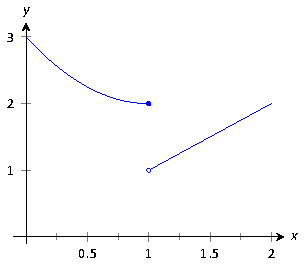
\includegraphics{test-figure2.pdf}
%  \captionof{figure}{Test caption}
%  \end{minipage}}}


%\newenvironment{mfigurefile}[2]{%
%\begin{tikzpicture}[remember picture,overlay]%
%\ifthenelse{\isodd{\thepage}}{\node [xshift=-36pt-.5\marginparwidth,yshift=#2\paperheight] at (current page.south east) }{\node [xshift=36pt+.5\marginparwidth,yshift=#2\paperheight] at (current page.south west) }%
%{\input{#1}};}%
%{\end{tikzpicture}%
%}

%\DeclareCaptionType{mytype}[Typename][List of mytype]


    
%%%%
%% End margin figure 
%%%%    
    

\newcommand{\bmx}[1]{\left[\hskip -3pt\begin{array}{#1} }
\newcommand{\emx}{\end{array}\hskip -3pt\right]}

\newcommand{\btz}{\begin{center}\begin{tikzpicture}}
\newcommand{\etz}{\end{tikzpicture}\end{center}}

\newcommand{\ds}{\displaystyle}

\newcommand{\fp}{\ensuremath{f\,'}}
\newcommand{\fpp}{\ensuremath{f\,''}}

\newcommand{\Fp}{\ensuremath{F\primeskip'}}
\newcommand{\Fpp}{\ensuremath{F\primeskip''}}

\newcommand{\yp}{\ensuremath{y\primeskip'}}
\newcommand{\gp}{\ensuremath{g\primeskip'}}

\newcommand{\dx}{\ensuremath{\Delta x}}
\newcommand{\dy}{\ensuremath{\Delta y}}
%\newcommand{\dz}{\ensuremath{\Delta z}}
\newcommand{\ddz}{\ensuremath{\Delta z}}

\newcommand{\thet}{\ensuremath{\theta}}
\newcommand{\norm}[1]{\ensuremath{||\ #1\ ||}}
\newcommand{\vnorm}[1]{\ensuremath{\norm{\vec #1}}}
\newcommand{\snorm}[1]{\ensuremath{\left|\left|\ #1\ \right|\right|}}
\newcommand{\la}{\left\langle}
\newcommand{\ra}{\right\rangle}
\newcommand{\dotp}[2]{\ensuremath{\vec #1 \cdot \vec #2}}
\newcommand{\proj}[2]{\ensuremath{\text{proj}_{\,\vec #2}{\,\vec #1}}}
\newcommand{\crossp}[2]{\ensuremath{\vec #1 \times \vec #2}}
\newcommand{\veci}{\ensuremath{\vec i}}
\newcommand{\vecj}{\ensuremath{\vec j}}
\newcommand{\veck}{\ensuremath{\vec k}}
\newcommand{\vecu}{\ensuremath{\vec u}}
\newcommand{\vecv}{\ensuremath{\vec v}}
\newcommand{\vecw}{\ensuremath{\vec w}}
\newcommand{\vecx}{\ensuremath{\vec x}}
\newcommand{\vecy}{\ensuremath{\vec y}}
\newcommand{\vrp}{\ensuremath{\vec r\, '}}
\newcommand{\vsp}{\ensuremath{\vec s\, '}}
\newcommand{\vrt}{\ensuremath{\vec r(t)}}
\newcommand{\vst}{\ensuremath{\vec s(t)}}
\newcommand{\vvt}{\ensuremath{\vec v(t)}}
\newcommand{\vat}{\ensuremath{\vec a(t)}}
\newcommand{\px}{\ensuremath{\partial x}}
\newcommand{\py}{\ensuremath{\partial y}}
\newcommand{\pz}{\ensuremath{\partial z}}
\newcommand{\pf}{\ensuremath{\partial f}}
\newcommand{\underlinespace}{\underline{\phantom{xxxxxx}}}

\newcommand{\surfaceS}{\ensuremath{\mathcal{S}}}

\newcommand{\mathN}{\ensuremath{\mathbb{N}}}

\newcommand{\zerooverzero}{\ensuremath{\ds \raisebox{8pt}{\text{``\ }}\frac{0}{0}\raisebox{8pt}{\text{\ ''}}}}


\newcommand{\myrule}{\rule[-4pt]{0pt}{13pt}}
\newcommand{\mmrule}{\rule[-10pt]{0pt}{15pt}}
\newcommand{\myds}{\ds\mmrule}
\newcommand{\deriv}[2]{\ensuremath{\myds\frac{d}{dx}\left(#1\right)=#2}}
\newcommand{\myint}[2]{\ensuremath{\myds\int #1\ dx=} \ensuremath{\ds #2}}

\DeclareMathOperator{\sech}{sech}
\DeclareMathOperator{\csch}{csch}
\DeclareMathOperator{\curl}{curl}
\DeclareMathOperator{\divv}{div}

\newcommand{\sword}[1]{\textbf{#1}}

\newcommand{\primeskip}{\hskip.75pt}

%%%% Begin Header TikZ

%  Some TiKZ  shortcuts to help make drawing 3D vectors faster.
%

\newcommand{\plotlinecolor}{blue}

%
% Draw x and y tick marks
%
\newcommand{\drawxticks}[1]
{\foreach \x in {#1}
		{\draw  (\x,-.1)--(\x,.1);
			};
}
\newcommand{\drawyticks}[1]
{\foreach \x in {#1}
		{\draw  (-.1,\x)--(.1,\x);
			};
}

\newcommand{\drawxlines}[3]
{\draw[<->] (#1,0) -- (#2,0) node [right] {$x$};
\foreach \x in {#3}
		{\draw  (\x,-.1)--(\x,.1);
			};
}

\newcommand{\drawylines}[3]
{\draw[<->] (0,#1) -- (0,#2) node [above] {$y$};
\foreach \x in {#3}
		{\draw  (-.1,\x)--(.1,\x);
			};
}

\newcommand{\drawxlabels}[1]
{\foreach \x in {#1}
		{\draw  (\x,-.1) node [below] {\scriptsize $\x$};
		};
}

\newcommand{\drawylabels}[1]
{\foreach \x in {#1}
		{\draw  (-.1,\x) node [left] {\scriptsize $\x$};
		};
}

%% draw a box of margin width size to see if figure is properly contained within
\newcommand{\marginsizebox}{\draw (0,0)--(\marginparwidth,0)--(\marginparwidth,3)--(0,3)--cycle;}

%%%%
%%%%

\newcommand{\asyouread}[1]{\begin{tikzpicture}
\ifthenelse{\boolean{in_color}}{\node [preaction={fill=black,opacity=.5,transform canvas={xshift=1mm,yshift=-1mm}}, right color=blue!80!black!30, left color=blue!80] at (0,0) {\textcolor{white}{\textsf{\textit{AS YOU READ $\ldots$}}}};}
{\node [preaction={fill=black,opacity=.5,transform canvas={xshift=1mm,yshift=-1mm}}, right color=black!30, left color=black!10] at (0,0) {\textcolor{white}{\textsf{\textit{AS YOU READ $\ldots$}}}};}
\end{tikzpicture}
\begin{enumerate}
#1
\end{enumerate}
\vskip 20pt}

%%%%
%%  A new figure environment, trying to fix the float problem.
%%
%%%%

%\newcounter{myfigurecounter}[chapter]
%\renewcommand\themyfigurecounter{\thechapter.\arabic{myfigurecounter}}
%\newenvironment{myfigure}{\refstepcounter{myfigurecounter}}{}
%\newcommand{\mycaption}[1]{%
%\begin{center}%
%\vskip -1.5\baselineskip
%\begin{tikzpicture}%
%\draw (0,0) node [text width=\textwidth,align=center] {Figure \themyfigurecounter: #1};%
%\end{tikzpicture}%
%\end{center}%
%}
\ifthenelse{\boolean{xetex}}%
	{\sffamily
	%%\usepackage{fontspec}
	\usepackage{mathspec}
	\setallmainfonts[Mapping=tex-text]{Calibri}
	\setmainfont[Mapping=tex-text]{Calibri}
	\setsansfont[Mapping=tex-text]{Calibri}
	\setmathsfont(Greek){[cmmi10]}}
	{}
\fancyhead{}
\fancyfoot{}
\fancyhf{}
%\fancyfoot{\thepage}
%\fancyhead{\thepage}
\pagestyle{plain}

\begin{document}

\noindent\large\textbf{Chapter 1: Limits}\normalsize\\

We start with the limit def. of a function of two variables (easily extended to three/more). Matches (in meaning, not in wording) the definition given by Stewart. Thomas is similar but the set is defined to be the domain of $f$, though the point can be a boundary point of the domain (which implies, but doesn't require, that $P$ might not be part of the set). Larson/Edwards states that $P$ must be in an open ball on which $f$ is defined, though possibly not at $P$. Taalman/Kohn doesn't specify the set on which $f$ is defined, etc., at all. 

\definition{def:multilimita}{Limit of a Function of Two Variables}
{Let $S$ be a set containing $P=(x_0,y_0)$ where every open disk centered at $P$ contains points in $S$ other than $P$, let $f$ be a function of two variables defined on $S$, except possibly at $P$, and let $L$ be a real number. 
%Let $f(x,y)$ be a function of two variables and let $(x_0,y_0)$ be a point in the domain of $f$. 
The \sword{limit of $f(x,y)$ as $(x,y)$ approaches $(x_0,y_0)$ is $L$}, denoted $$\ds \lim_{(x,y)\to (x_0,y_0)} f(x,y) = L,$$
means that given any $\epsilon>0$, there exists $\delta>0$ such that for all  $(x,y)$ in $S$, where $(x,y)\neq (x_0,y_0)$, if $(x,y)$ is in the open disk centered at $(x_0,y_0)$ with radius $\delta$, then $|f(x,y) - L|<\epsilon.$
\index{limit!of multivariable function}\index{multivariable function!limit}
}


A key phrase is ``all $(x,y)$ in $S$''. Allows for limits at the boundary of $S$. Larson/Edwards uses ``all $(x,y)$ in open ball centered at $(x_0,y_0)$ ...'' but later gives limits such as
$$\lim_{(x,y)\to (0,0)} \frac{x+y}{x^2+y},$$
where the function is not defined on all points in any open ball containing $(0,0)$, therefore technically we can't take the limit. (See note in 12.2 section later.)

The natural constriction of this definition to functions of one variable is given below, which doesn't match any texts I've seen. Key phrase: ``for all $x$ in $I$''.

\definition{def:limit}{The Limit of a Function of One Variable}
{Let $I$ be an interval containing $c$, let $f$ be a function defined on $I$, except possibly at $c$, and let $L$ be a real number. The \sword{limit of $f(x)$ as $x$ approaches $c$ is $L$}, denoted by  
$$\displaystyle \lim_{x\rightarrow c} f(x) = L,$$
means that given any $\epsilon > 0$, there exists $\delta > 0$ such that for all $x$ in $I$, where $x\neq c$,  
if  $|x - c| < \delta$, then $|f(x) - L| < \epsilon$.\index{limit!definition}
}

As before, this allows for finding ``the'' limit at the boundary/endpoint of $I$.

The following is the current APEX def of the left-hand limit. It is wrong; $c$ is in an open interval $(a,b)$, therefore it doesn't allow for finding limit from the left at $x=b$. 

\definition{def:onesidedlimitold}{One Sided Limits}
{\textbf{Left-Hand Limit} \index{limit!one sided}\index{limit!right handed}\index{limit!left handed}

\indent Let $I$ be an open interval containing $c$, and let $f$ be a function defined on $I$, except possibly at $c$. 
The \sword{limit of $f(x)$, as $x$ approaches $c$ from the left, is $L$}, or, \sword{the left--hand limit of $f$ at $c$ is $L$}, denoted by  
$$\displaystyle \lim_{x\rightarrow c^-} f(x) = L,$$
means that given any $\epsilon > 0$, there exists $\delta > 0$ such that for all $x< c$,  
if  $|x - c| < \delta$, then $|f(x) - L| < \epsilon$.
}

A proposed correction, which is similar to Thomas, though the Thomas definition lacks rigor. Larson/Edwards has a heuristic definition, stated informally within a discussion.

\definition{def:onesidedlimit}{One Sided Limits}
{\textbf{Left-Hand Limit} \index{limit!one sided}\index{limit!right handed}\index{limit!left handed}

\indent Let $f$ be a function defined on $(a,c)$ for some $a<c$ and let $L$ be a real number. 

The \sword{limit of $f(x)$, as $x$ approaches $c$ from the left, is $L$}, or, \sword{the left--hand limit of $f$ at $c$ is $L$}, denoted by  
$$\displaystyle \lim_{x\rightarrow c^-} f(x) = L,$$
means that given any $\epsilon > 0$, there exists $\delta > 0$ such that for all $a<x<c$,  
if  $|x - c| < \delta$, then $|f(x) - L| < \epsilon$.
}

This is a natural restriction of the limit def. to a one-sided limit. The key phrase ``for all $x$ in $I$'' from the limit definition is replaced with a simple $a<x<c$. Note also $|x-c|$ can be construed as unnecessary; we could write ``$c-x$'', but it is kept to model previous definitions. Opens up an opportunity for an exercise. The right hand limit would be defined similarly.

The change to ``the'' limit definition doesn't change the following theorem, as it is given on an open interval. Some of the content following may need to change; perhaps highlight the fact that we are only talking of points within an open interval.

\theorem{thm:leftrightlimits}{Limits and One Sided Limits}
{Let $f$ be a function defined on an open interval $I$ containing $c$ and let $L$ be a real number. \index{limit!does not exist} Then $$\lim_{x\to c}f(x) = L$$ if, and only if, $$\lim_{x\to c^-}f(x) = L \quad \text{and} \quad \lim_{x\to c^+}f(x) = L.$$}

In Section 1.3, need to change part 8 to be more precise, matching limit thm in Chapter 12. (Check also emails for errata on \# 9)

\theorem{thm:limit_algebra}{Basic Limit Properties}{\small
Let $b$, $c$, $L$ and $K$ be real numbers, let $n$ be a positive integer, and let $f$ and $g$ be functions defined on an interval $I$ containing $c$ with the following limits: \index{limit!properties}
$$\lim_{x\to c}f(x) = L \text{\ and\ } \lim_{x\to c} g(x) = K.$$
The following limits hold.
\begin{enumerate}
\item \parbox{80pt}{Constants:} $\displaystyle \lim_{x\to c} b = b$
\item	\parbox{80pt}{Identity }						$\displaystyle \lim_{x\to c} x = c$
\item	\parbox{80pt}{Sums/Differences:} $\displaystyle \lim_{x\to c}\big(f(x)\pm g(x)\big) = L\pm K$
\item	\parbox{80pt}{Scalar Multiples:}	$\displaystyle \lim_{x\to c} \big(b\cdot f(x) \big)= bL$
\item	\parbox{80pt}{Products:}	$\displaystyle \lim_{x\to c} \big(f(x)\cdot g(x)\big) = LK$
\item	\parbox{80pt}{Quotients:} $\displaystyle \lim_{x\to c} \big(f(x)/g(x)\big) = L/K$, (where $K\neq 0)$
\item	\parbox{80pt}{Powers:} 	$\displaystyle \lim_{x\to c} \big(f(x)^n\big) = L^n$
\item	\parbox{80pt}{Roots:}		\parbox[t]{185pt}{$\displaystyle \lim_{x\to c} \sqrt[n]{f(x)} = \sqrt[n]{L}$ \par \small (If $n$ is even then require $f(x)\geq 0$ on $I$.)}
\item	\parbox{80pt}{Compositions:} \parbox[t]{200pt}{Adjust our previously given limit situation to: $$\lim_{x\to c}f(x) = L,\ \lim_{x\to L} g(x) = K \text{\ and\ } g(L)=K .$$ Then $\ds \lim_{x\to c}g(f(x)) = K$.}
\end{enumerate}
}

The definition of continuity changes to remove the restriction of an open interval. This allows for continuity on a closed interval. We effectively get to this point later, anyway, by incorporating left/right hand limits on closed intervals. This will immediately change the outcome of the example in the text following the definition. This will actually remove some ambiguity; in that example, we state that a function is continuous on $(0,1)$ and $(1,3)$, whereas later we would have said $[0,1)$ and $(1,3]$ once we defined continuity at an endpoint.

\definition{def:continuous}{Continuous Function}
{Let $f$ be a function defined on an interval $I$ containing $c$. \index{continuous function} 
	\begin{enumerate}
	\item		$f$ is \textbf{continuous at $c$} if $\ds \lim_{x\to c}f(x) = f(c)$.
	\item		$f$ is \textbf{continuous on $I$} if $f$ is continuous at $c$ for all values of $c$ in $I$. If $f$ is continuous on $(-\infty,\infty)$, we say $f$ is \textbf{continuous everywhere}.
	\end{enumerate}
}

We now remove the following definition from the book, as it is unnecessary.

\definition{def:closed_continuity}{Continuity on Closed Intervals}
{Let $f$ be defined on the closed interval $[a,b]$ for some real numbers $a,b$. $f$ is \textbf{continuous on $[a,b]$} if:
		\begin{enumerate}
		\item		$f$ is continuous on $(a,b)$,
		\item		$\ds \lim_{x\to a^+} f(x) = f(a)$ and 
		\item		$\ds \lim_{x\to b^-} f(x) = f(b)$.
		\end{enumerate}
		}
		
We have always wanted continuity on a closed interval; we now have it by ``initial'' definition, not by ``additional'' definition. We use continuity on a closed interval for the Intermediate Value Theorem, which does not change.

Limits at $c$ that involve infinity needs to change. The current APEX definition is ok in spirit, but imprecise. It doesn't give a domain for $f$. (Thomas actually doesn't formally define this limit; it is discussed in a paragraph. Larson/Edwards defines this limit formally on open intervals.) Suggested change, which formally adds limit approaching $-\infty$:

\definition{def:limit_of_infinity}{Limit of Infinity, $\infty$, Vertical Asymptote}
{Let $I$ be an interval containing $c$, and let $f$ be a function defined on $I$, except possibly at $c$. \begin{itemize}
	\item We say \sword{the limit of $f(x)$, as $x$ approaches $c$, is infinity}, denoted by $\ds \lim_{x\rightarrow c} f(x)=\infty$, if for every $N>0$ there exists $\delta>0$ such that for all $x$ in $I$, where $x\neq c$, if  $|x-c|<\delta$, then $f(x)> N$. \index{limit!of infinity}  
	\item	We say \sword{the limit of $f(x)$, as $x$ approaches $c$, is negative infinity}, denoted by $\ds \lim_{x\rightarrow c} f(x)=-\infty$, if for every $N<0$ there exists $\delta>0$ such that for all $x$ in $I$, where $x\neq c$, if  $|x-c|<\delta$, then $f(x)<N$. \index{limit!of infinity}  
	\item	If $\ds \lim_{x\rightarrow c} f(x)=\pm\infty$, we say the line $x=c$ is a \sword{vertical asymptote} of $f$.\index{asymptote!vertical}
\end{itemize}
}
		
Note that this allows for $c$ to be an endpoint of $I$; it does not need one-sided limits. Allows us to immediately say that $x=0$ is a vertical asymptote of $\ln x$.

The current APEX does not formally define vertical asymptotes, though it does in a paragraph. It formally defines horizontal asymptotes so this change aligns well.


The definition of limits at infinity are ok in spirit but need to be made more precise.

\definition{def:limit_at_infinity}{Limits at Infinity and Horizontal Asymptote}
{Let $L$ be a real number.
\begin{enumerate}
\item Let $f$ be a function defined on $(a,\infty)$ for some number $a$. We say $\ds\lim_{x\rightarrow\infty} f(x)=L$ if for every $\epsilon>0$ there exists $M>a$ such that if $x > M$, then $|f(x)-L|<\epsilon$.\index{limit!at infinity}\index{asymptote!horizontal} \\

\item Let $f$ be a function defined on $(-\infty,b)$ for some number $b$. We say $\ds\lim_{x\rightarrow-\infty} f(x)=L$ if for every $\epsilon>0$ there exists $M<b$ such that if $x < M$, then $|f(x)-L|<\epsilon$. \\

 \item  If $\ds\lim_{x\rightarrow\infty} f(x)=L$ or $\ds\lim_{x\rightarrow-\infty} f(x)=L$, we say the line $y=L$ is a \sword{horizontal asymptote} of $f$.
\end{enumerate}
}
Will add a line to the text and an exercise along the lines of ``We can combine definitions 7 \& 8 to give meaning to the expression `$\lim_{x\to\infty}f(x) = \infty$.' We leave this to the reader as a problem in the Exercises.''\\

\noindent\large\textbf{Chapter 2: Derivatives}\normalsize\\

This chapter begins with an example of approximating the velocity of a falling object when it lands. Strictly speaking, by our old definitions of limits (and derivatives), our answer should be ``We don't know as we can't find the derivative at the endpoint of an interval.''

A new definition of derivative: $I$ is no longer an open interval (that was required by the limit definition). Opens the door for the derivative at the endpoint.

\definition{def:derivative_at_a_point}{Derivative at a Point}{Let $f$ be a continuous function on an  interval $I$ containing $c$.\index{derivative!at a point} The \sword{derivative of $f$ at $c$}, denoted $\fp(c)$, is $$\lim_{h\to 0}\frac{f(c+h)-f(c)}{h},$$ provided the limit exists. If the limit exists, we say that \sword{$f$ is differentiable at $c$}; if the limit does not exist, then \sword{$f$ is not differentiable at $c$}. If $f$ is differentiable at every point in $I$, then \sword{$f$ is differentiable on $I$}.\index{differentiable}
}

This changes the definitions of tangent/normal lines by not restricting to open intervals. We may as well go further: instead of ``Let $f$ be continuous on an  interval $I$ and differentiable at $c$, for some $c$ in $I$.'' we can say ``Let $f$ be a differentiable function on an interval $I$ containing $c$.'', as done below.

\definition{def:tangent_line}{Tangent Line}{Let $f$ be a differentiable function on an interval $I$ containing $c$. The line with equation $\ell(x) = \fp(c)(x-c)+f(c)$ is the \textbf{tangent line} to the graph of $f$ at $c$; that is, it is the line through $(c,f(c))$ whose slope is the derivative of $f$ at $c$.\index{tangent line}\index{derivative!tangent line}}

\definition{def:normal_line}{Normal Line}
{Let $f$ be a differentiable function on an interval $I$ containing $c$. The \textbf{normal line} to the graph of $f$ at $c$ is the line with equation
$$n(x) =\frac{-1}{\fp(c)}(x-c)+f(c),$$ where $\fp(c)\neq 0$. When $\fp(c)=0$, the normal line is the vertical line through $\big(c,f(c)\big)$; that is, $x=c$.\index{derivative!normal line}\index{normal line}
}

Next is the definition of the derivative function; we again remove the open interval restriction.

\definition{def:the_derivative}{Derivative Function}
{Let $f$ be a differentiable function on an  interval $I$. The function $$\fp(x) = \lim_{h\to 0} \frac{f(x+h)-f(x)}{h}$$ is \sword{the derivative of $f$}.\index{derivative!as a function}\index{derivative!notation}\\

\sword{Notation:} 

Let $y = f(x)$. The following notations all represent the derivative of $f$\,:
$$\fp(x)\ =\ y\,'\ =\ \frac{dy}{dx}\ =\ \frac{df}{dx}\ =\ \frac{d}{dx}(f)\ =\ \frac{d}{dx}(y). $$}

Nothing in Section 2.2 changes. In Section 2.3, we use ``an interval'' as before. 

\theorem{thm:deriv_prop}{Properties of the Derivative}
{Let $f$ and $g$ be differentiable functions on an interval $I$ and let $c$ be a real number. Then:
	\begin{enumerate}
	%\item		\parbox{75pt}{\textbf{Sum/Difference Rule:}}\parbox[t]{176pt}{$\ds \frac{d}{dx}\Big(f(x) \pm g(x)\Big) = \frac{d}{dx}\Big(f(x)\Big) \pm \frac{d}{dx}\Big(g(x)\Big)$ $= \rule{0pt}{15pt}\fp(x)\pm g\primeskip'(x)$}
	\item	\sword{Sum/Difference Rule:}
	
	$\ds \frac{d}{dx}\Big(f(x) \pm g(x)\Big) = \frac{d}{dx}\Big(f(x)\Big) \pm \frac{d}{dx}\Big(g(x)\Big)$ $= \rule{0pt}{15pt}\fp(x)\pm g\primeskip'(x)$
	\index{derivative!Sum/Difference Rule}\index{Sum/Difference Rule!of derivatives}
	\item		\sword{Constant Multiple Rule:}
	
	$\ds \frac{d}{dx}\Big(c\cdot f(x)\Big) = c\cdot\frac{d}{dx}\Big(f(x)\Big) = c\cdot\fp(x)$.\index{derivative!Constant Multiple Rule}\index{Constant Multiple Rule!of derivatives}
	\end{enumerate}
}

\definition{def:Higher_Deriv}{Higher Order Derivatives}
{Let $y=f(x)$ be a differentiable function on an interval $I$. \index{derivative!higher order}\index{derivative!notation}
		\begin{enumerate}
		\item		The \textit{second derivative} of $f$ is: 
						$$ \fp'(x) = \frac{d}{dx}\Big(\fp(x)\Big) = \frac{d}{dx}\left(\frac{dy}{dx}\right) = \frac{d\primeskip^2y}{dx^2}=y\primeskip''.$$
				\item		The \textit{third derivative} of $f$ is: 
						$$ \fp''(x) = \frac{d}{dx}\Big(\fp'(x)\Big) = \frac{d}{dx}\left(\frac{d\primeskip^2y}{dx^2}\right) = \frac{d\primeskip^3y}{dx^3}=y\primeskip'''.$$
				\item		The \textit{n$^{\text{th}}$ derivative} of $f$ is:
						$$ f\,^{(n)}(x) = \frac{d}{dx}\left(f\,^{(n-1)}(x)\right) = \frac{d}{dx}\left(\frac{d\primeskip^{n-1}y}{dx^{n-1}}\right) = \frac{d\primeskip^ny}{dx^n}=y^{(n)}.$$
		\end{enumerate}
}

There is a marginal note for this last definition that gives the caveat ``where the corresponding limits exist.'' It is a necessary note, but not needed in the definition, per se.

Section 2.4: Remove ``open''.

\theorem{thm:ProductRule}{Product Rule}
{Let $f$ and $g$ be differentiable functions on an  interval $I$.\index{Power Rule!differentiation}\index{derivative!Product Rule} Then $fg$ is a differentiable function on $I$, and $$\frac{d}{dx}\Big(f(x)g(x)\Big) = f(x)g\primeskip'(x) + \fp(x)g(x).$$}

The APEX Quotient rule wasn't good. $f$ and $g$ were ``functions defined on an open interval $I$, not even mentioning that they were differentiable.

\theorem{thm:QuotientRule}{Quotient Rule}
{Let $f$ and $g$ be differentiable functions on an interval $I$, where $g(x) \neq 0$ on $I$.\index{derivative!Quotient Rule}\index{Quotient Rule} Then $f/g$ is differentiable on $I$, and $$\frac{d}{dx}\left(\frac{f(x)}{g(x)}\right) = \frac{g(x)\fp(x) - f(x)g\primeskip'(x)}{g(x)^2}.$$
}

Section 2.5: The definition of the Chain Rule needed some cleaning up anyway to talk about the domains of the functions. It gets a bit wordy.

\theorem{thm:chain_rule}{The Chain Rule}
{Let $g$ be a differentiable function on an interval $I$, let the range of $g$ be a subset of the interval $J$, and let $f$ be a differentiable function on $J$.
\index{derivative!Chain Rule}\index{Chain Rule} Then $y=f(g(x))$ is a differentiable function on $I$, and $$y\primeskip' = \fp(g(x))\cdot g\primeskip'(x).$$
}

\theorem{thm:gen_power_rule}{Generalized Power Rule}{Let $g(x)$ be a differentiable function on an interval $I$ and let $n\neq 0$ be an integer.\index{derivative!Generalized Power Rule}\index{Generalized Power Rule} Then $g(x)^n$ is differentiable on $I$, and $$\frac{d}{dx}\Big(g(x)^n\Big) = n\cdot \big(g(x)\big)^{n-1}\cdot g\primeskip'(x).$$
}

Slight rewording here, using ``differentiable everywhere'':

\theorem{thm:exponentials}{Derivatives of Exponential Functions}
{Let $f(x)=a^x$, for $a>0$ and $a\neq 1$.\index{derivative!exponential functions} Then $f$ is differentiable everywhere and $$\fp(x) = \ln a\cdot a^x.$$
}

2.6: Implicit Differentiation gives a final version of the Power Rule. Changed to ``diff on its domain except possibly at $x=0$.''

\theorem{thm:finalpower}{Power Rule for Differentiation}
{Let $f(x) = x^n$, where $n\neq 0$ is a real number. Then $f$ is differentiable on its domain, except possibly at $x=0$, and $\fp(x) = n\cdot x^{n-1}$.\index{derivative!Power Rule}\index{Power Rule!differentiation}
}



2.7: Inverse Functions. The original theorem restricts to open intervals which we remove here. In practice, open intervals are the result of one-to-one functions on as large an interval as possible, as, for instance, $f(x) = \sin x$ is one to one on $[-\pi/2,\pi/2]$ but has $f\,'(x) = 0$ at the endpoints.

\theorem{thm:deriv_inverse_functions}{Derivatives of Inverse Functions}
{Let $f$ be differentiable and one to one on an interval $I$, where $\fp(x) \neq 0$ for all $x$ in $I$, let $J$ be the range of $f$ on $I$, let $g$ be the inverse function of $f$, and let $f(a) = b$ for some $a$ in $I$. Then $g$ is a differentiable function on $J$, and in particular,
	
%	\begin{center}
\hskip-7pt	\begin{tabular}{ccc}
	1. $\ds \left(f\primeskip^{-1}\right)'(b)=g\primeskip'(b) = \frac{1}{\fp(a)}$ &\hskip 4pt and \hskip 4pt&  2. $\ds \left(f\primeskip^{-1}\right)'(x)=g\primeskip'(x) = \frac{1}{\fp(g(x))}$
	\end{tabular}
%	\end{center}
}

The following theorem will be unchanged. It does specify open sets, but this is also specific to these functions. Some have closed domains, but they are not differentiable at their endpoints.

\theorem{thm:deriv_inverse_trig}{Derivatives of Inverse Trigonometric Functions}
{The inverse trigonometric functions are differentiable on all open sets contained in their domains (as listed in Figure \ref{fig:domain_trig}) and their derivatives are as follows:\\

\noindent	\begin{minipage}{.5\specialboxlength}\small
	\begin{enumerate}
	\item		$\ds \frac{d}{dx}\big(\sin^{-1}(x)\big) = \frac{1}{\sqrt{1-x^2}}$ 
	\item		$\ds \frac{d}{dx}\big(\sec^{-1}(x)\big) = \frac{1}{|x|\sqrt{x^2-1}}$
	\item		$\ds \frac{d}{dx}\big(\tan^{-1}(x)\big) = \frac{1}{1+x^2}$
	\end{enumerate}
	\end{minipage}
	\begin{minipage}{.5\specialboxlength}\small
	\begin{enumerate}\addtocounter{enumi}{3}
	\item		$\ds \frac{d}{dx}\big(\cos^{-1}(x)\big) = -\frac{1}{\sqrt{1-x^2}}$ 
	\item		$\ds \frac{d}{dx}\big(\csc^{-1}(x)\big) = -\frac{1}{|x|\sqrt{x^2-1}}$
	\item		$\ds \frac{d}{dx}\big(\cot^{-1}(x)\big) = -\frac{1}{1+x^2}$
	\end{enumerate}\index{derivative!inverse trig.}
	\normalsize
	\end{minipage}
}			

\noindent\large\textbf{Chapter 3: Graphical Behavior of Functions}\normalsize\\

3.1: Extreme Values

The definition of the extreme values (absolute max/min) does not change. The Extreme Value Theorem does not change.

The definition of Relative Max/Min changes. It was always defined on an interval $I$ (not necessarily open).  Allows for a rel max/min to occur at an endpoint. Examples and exercises will need to be changed to follow.

\definition{def:rel_ext}{Relative Minimum and Relative Maximum}%
{Let $f$ be defined on an interval $I$ containing $c$. 
		\begin{enumerate}
		\item	If there is a $\delta>0$ such that $f(c) \leq f(x)$ for all $x$ in $I$ where $|x-c|<\delta$, then $f(c)$ is a \sword{relative minimum} of $f$. We also say that $f$ has a relative minimum at $(c,f(c))$. \index{minimum!relative/local}\index{extrema!relative}
		
		\item	If there is a $\delta>0$ such that $f(c) \geq f(x)$ for all $x$ in $I$ where $|x-c|<\delta$, then $f(c)$ is a \sword{relative maximum} of $f$. We also say that $f$ has a relative maximum at $(c,f(c))$. \index{maximum!relative/local}\index{extrema!relative}
		\end{enumerate}
		
The relative maximum and minimum values comprise the \textbf{relative extrema} of $f$.
}

The definition of a critical number/point does not change. 

The following theorem is rewritten to specify we only consider rel extrema on open intervals.

\theorem{thm:criticalpts}{Relative Extrema and Critical Points}
{Let a function $f$ be defined on an open interval $I$ containing $c$, and let $f$ have a relative extrema at the point $(c,f(c))$. Then $c$ is a critical number of $f$.
}

The subsequent Key Idea on finding abs. extrema on a closed interval does not change.\\


3.2: The Mean Value Theorem

The Mean Value Thm and Rolle's Thm do not change. Both specify continuous on $[a,b]$ and diff. on $(a,b)$ which is wanted; we don't need to require differentiability at the endpoints. \\

3.3 Increasing and Decreasing Functions

The definitions of increasing/decreasing are a bit of a mess. We remove ``strictly incr/decr'' and exchage the ``$\leq$'' for ``$<$'', etc.

\definition{def:incr_decr}{Increasing and Decreasing Functions}
{Let $f$ be a function defined on an interval $I$.\index{increasing function}\index{decreasing function}\index{increasing function!strictly}\index{decreasing function!strictly}
\begin{enumerate}
\item		$f$ is \textbf{increasing} on $I$ if for every $a<b$ in $I$, $f(a) < f(b)$.
\item		$f$ is \textbf{decreasing} on $I$ if for every $a<b$ in $I$, $f(a) > f(b)$.
\end{enumerate}
}

The theorem following this definition is now correct; if $f\,'(x) > 0$, then $f$ is increasing. The Key Idea that follows is also fine. The first derivative test is fine.\\

3.4/3.5: Concavity and the Second Derivative/Curve Sketching

All theorems and defs here are not affected by the changes.\\

\noindent\large\textbf{Chapter 4: Applications of the Derivatives}\normalsize\\

No changes are needed. \\

\noindent\large\textbf{Chapter 5: Integration}\normalsize\\

The Fundamental Theorem of Calc changes to be diff. on the closed interval.

\theorem{thm:FTC1}{The Fundamental Theorem of Calculus, Part 1}
{Let $f$ be continuous on $[a,b]$ and let $\ds F(x) = \int_a^x f(t)\ dt$. Then $F$ is a differentiable function on $[a,b]$, and\index{Fundamental Theorem of Calculus}\index{integration!Fun. Thm. of Calc.} $$\Fp(x)=f(x).$$
}

The rest of chapter 5 is unchanged.\\

\noindent\large\textbf{Chapter 6: Antidifferentiation}\normalsize\\

L'H\^opital's Rule (both parts) changes to remove the word ``open'' as before with limits. In ``Part 2 of Part 2'', we leave the word open because it really doesn't matter if the interval is $(a,\infty)$ or $[a,\infty)$. Added quotes to the indeterminate forms in that part, too.

\theorem{thm:LHR}{L'H\^opital's Rule, Part 1}
{Let $\ds \lim_{x\to c}f(x) = 0$ and $\ds \lim_{x\to c}g(x)=0$, where $f$ and $g$ are differentiable functions on an interval $I$ containing $c$, and let $g\primeskip'(x)\neq 0$ on $I$ except possibly at $c$. Then \index{limit!L'H\^opital's Rule}\index{L'H\^opital's Rule}
$$ \lim_{x\to c} \frac{f(x)}{g(x)} = \lim_{x\to c} \frac{\fp(x)}{g\primeskip'(x)}.$$
}

\theorem{thm:LHR2}{L'H\^opital's Rule, Part 2}
{\begin{enumerate}
\item		Let $\ds\lim_{x\to a}f(x) = \pm\infty$ and $\ds\lim_{x\to a}g(x)=\pm \infty$, where $f$ and $g$ are differentiable on an interval $I$ containing $a$. Then \index{limit!L'H\^opital's Rule}\index{L'H\^opital's Rule}
$$\lim_{x\to a} \frac{f(x)}{g(x)} = \lim_{x\to a}\frac{\fp(x)}{g\primeskip'(x)}.$$

\item		Let $f$ and $g$ be differentiable functions on the open interval $(a,\infty)$ for some value $a$, where $g\primeskip'(x)\neq 0$ on $(a,\infty)$ and $\ds\lim_{x\to\infty} f(x)/g(x)$ returns either ``0/0'' or ``$\infty/\infty$''. Then
$$\lim_{x\to \infty} \frac{f(x)}{g(x)} = \lim_{x\to \infty}\frac{\fp(x)}{g\primeskip'(x)}.$$
A similar statement can be made for limits where $x$ approaches $-\infty$.
\end{enumerate}
}

\noindent\large\textbf{Chapter 7: Applications}\normalsize\\


The Arc Length Key Idea should be elevated to a Theorem. Also, it states that $f$ should be diff. on an open interval containing $[a,b]$, but the first example is of the arc length of $f(x) = x^{3/2}$ on $[0,4]$. Changing wording to ``differentiable on $[a,b]$. Same holds for surface area of solid of revolution.

\theorem{thm:arclength}{Arc Length}
{Let $f$ be differentiable on $[a,b]$, where $\fp$ is also continuous on $[a,b]$. Then the arc length of $f$ from $x=a$ to $x=b$ is
\index{integration!arc length}\index{arc length}
$$L = \int_a^b \sqrt{1+\fp(x)^2}\ dx.$$
}

\theorem{thm:surface_area}{Surface Area of a Solid of Revolution}
{Let $f$ be differentiable on  $[a,b]$, where $\fp$ is also continuous on $[a,b]$. \index{integration!surface area}\index{surface area!solid of revolution}
	\begin{enumerate}
	\item	The surface area of the solid formed by revolving the graph of $y=f(x)$, where $f(x)\geq0$, about the $x$-axis is
	$$\text{Surface Area} = 2\pi\int_a^b f(x)\sqrt{1+\fp(x)^2}\ dx.$$
	\item	The surface area of the solid formed by revolving the graph of $y=f(x)$ about the $y$-axis, where $a,b\geq0$, is
	$$\text{Surface Area} = 2\pi\int_a^b x\sqrt{1+\fp(x)^2}\ dx.$$
	\end{enumerate}
}

Should Work and Fluid Force be given as Theorems or Key Ideas? They are currently Key Ideas. Volume found by integrating cross--sectional area is a Theorem; the subsequent Disk/Washer Methods are Key Ideas, as is the Shell Method. Should that change?\\

\noindent\large\textbf{Chapter 8:Sequences and Series}\normalsize\\

Removed the first statement which says ``bounded, monotonic sequences converge.'' All three are redundant. Will add the missing statement to the exercises.

\theorem{thm:monotonic_converge}{Bounded Monotonic Sequences are Convergent}
{\begin{enumerate}
%\item		Let $\{a_n\}$ be a bounded, monotonic sequence. Then $\{a_n\}$ converges; i.e., $\ds \lim_{n \to\infty}a_n$ exists.
\item		Let $\{a_n\}$ be a monotonically increasing sequence that is bounded above. Then $\{a_n\}$ converges.
\item		Let $\{a_n\}$ be a monotonically decreasing sequence that is bounded below. Then $\{a_n\}$ converges.
\index{sequences!convergent}\index{convergence!of monotonic sequences}
\end{enumerate}
}

8.2: Series\\
Renamed the following theorem to remove the idea of ``Convergence'' as it isn't a test for convergence, ever. Changed the order of the list to emphasize the more important idea.
\theorem{thm:series_nth_term}{$n^\text{th}$--Term Test for Divergence}
{Consider the series $\ds\sum_{n=1}^\infty a_n$. 
\index{series!nth@$n^\text{th}$--term test}\index{nth@$n^\text{th}$--term test}\index{convergence!nth@$n^\text{th}$--term test}\index{divergence!nth@$n^\text{th}$--term test}
\begin{enumerate}
\item		If $\ds \lim_{n\to\infty}a_n \neq 0$, then $\ds\sum_{n=1}^\infty a_n$ diverges.
\item		If $\ds\sum_{n=1}^\infty a_n$ converges, then $\ds \lim_{n\to\infty}a_n =0$.
\end{enumerate}
}

\noindent\large\textbf{Chapter 9: Curves in the plane}\normalsize\\

9.3: Calc and parametric equations\\

Remove ``open'' from following key ideas. Elevate to Theorems?

\keyidea{idea:dydxpar}{Finding $\frac{dy}{dx}$ with Parametric Equations.}
{Let $x=f(t)$ and $y=g(t)$, where $f$ and $g$ are differentiable functions on an interval $I$ and $\fp(t)\neq 0$ on $I$. Then \index{parametric equations!finding $\frac{dy}{dx}$}\index{derivative!parametric equations}
$$\frac{dy}{dx} = \frac{g\primeskip'(t)}{\fp(t)}.$$
}

\keyidea{idea:second_der_par}{Finding $\frac{d^2y}{dx^2}$ with Parametric Equations}
{Let $x=f(t)$ and $y=g(t)$ be twice differentiable functions on an interval $I$, where $\fp(t)\neq 0$ on $I$. Then 
\index{parametric equations!finding $\frac{d^2y}{dx^2}$}
$$\frac{d^2y}{dx^2}\quad = \quad\frac{d}{dt}\left[\frac{dy}{dx}\right]\Bigg/\frac{dx}{dt} \quad=\quad \frac{d}{dt}\left[\frac{dy}{dx}\right]\Bigg/\fp(t).$$ 
}

Change wording to match the previous arc length definition.

\theorem{thm:arc_length_parametric}{Arc Length of Parametric Curves}
{Let $x=f(t)$ and $y=g(t)$ be parametric equations with $\fp$ and $g\primeskip'$ continuous on $[t_1,t_2]$, on which the graph traces itself only once. The arc length of the graph, from $t=t_1$ to $t=t_2$, is
\index{parametric equations!arc length}\index{arc length}
$$L = \int_{t_1}^{t_2} \sqrt{\fp(t)^2+g\primeskip'(t)^2}\ dt.$$
}

Elevate to theorem, change wording to match:

\theorem{thm:surface_area_parametric}{Surface Area of a Solid of Revolution}
{Consider the graph of the parametric equations $x=f(t)$ and $y=g(t)$, where $\fp$ and $g\primeskip'$ are continuous on  $[t_1,t_2]$ on which the graph does not cross itself.\index{surface area!solid of revolution}\index{integration!surface area}\index{parametric equations!surface area}
\begin{enumerate}
	\item	The surface area of the solid formed by revolving the graph about the $x$-axis is (where $g(t)\geq~0$ on $[t_1,t_2]$):
	$$\text{Surface Area} = 2\pi\int_{t_1}^{t_2} g(t)\sqrt{\fp(t)^2+g\primeskip'(t)^2}\ dt.$$
	
	\item	The surface area of the solid formed by revolving the graph about the $y$-axis is (where $f(t)\geq~0$ on $[t_1,t_2]$):
	$$\text{Surface Area} = 2\pi\int_{t_1}^{t_2} f(t)\sqrt{\fp(t)^2+g\primeskip'(t)^2}\ dt.$$
	\end{enumerate}
\vskip-\baselineskip
}

9.5: Calc and polar functions\\

Elevate to theorem? Added an interval for definition of $f$.

\keyidea{idea:dydxpol}{Finding $\frac{dy}{dx}$ with Polar Functions}
{Let $r=f(\theta)$ be a polar function, where $f$ is differentiable on an interval $I$. With $x=f(\theta)\cos\theta$ and $y=f(\theta)\sin\theta$,
\index{polar!functions!finding $\frac{dy}{dx}$}\index{tangent line}
$$\frac{dy}{dx} = \frac{\fp(\theta)\sin\theta+f(\theta)\cos\theta}{\fp(\theta)\cos\theta-f(\theta)\sin\theta}.$$
}

Elevate to theorem, as both previous statements on areas between curves  and arc lengths and surface areas are theorems. Also change ``open'' language of arc length and surface area.

\theorem{thm:area_between_polar}{Area Between Polar Curves}
{The area $A$ of the region bounded by $r_1=f_1(\theta)$ and $r_2=f_2(\theta)$, $\theta=\alpha$ and $\theta=\beta$, where $f_1(\theta)\leq f_2(\theta)$ on $[\alpha,\beta]$, is
$$A = \frac12\int_\alpha^\beta \big(r_2^{\,2}-r_1^{\,2}\big)\ d\theta.$$
}

\theorem{thm:polar_arclength}{Arc Length of Polar Curves}
{Let  $r=f(\theta)$ be a polar function with $\fp$ continuous on $[\alpha,\beta]$, on which the graph traces itself only once. The arc length $L$ of the graph on $[\alpha,\beta]$ is
$$L = \int_\alpha^\beta \sqrt{\fp(\theta)^2+f(\theta)^2}\ d\theta = \int_\alpha^\beta\sqrt{(r\,')^2+ r^2}\ d\theta.$$
}

\theorem{thm:surface_area_polar}{Surface Area of a Solid of Revolution}
{Consider the graph of the polar equation $r=f(\theta)$, where $\fp$ is continuous on  $[\alpha,\beta]$ on which the graph does not cross itself.
\index{surface area!solid of revolution}\index{polar!function!surface area}\index{integration!surface area}
	\begin{enumerate}
		\item The surface area of the solid formed by revolving the graph about the initial ray ($\theta=0$) is:
		$$\text{Surface Area} = 2\pi\int_\alpha^\beta f(\theta)\sin\theta\sqrt{\fp(\theta)^2+f(\theta)^2}\ d\theta.$$
		\item The surface area of the solid formed by revolving the graph about the line $\theta=\pi/2$ is:
		$$\text{Surface Area} = 2\pi\int_\alpha^\beta f(\theta)\cos\theta\sqrt{\fp(\theta)^2+f(\theta)^2}\ d\theta.$$
	\end{enumerate}
}

\noindent\large\textbf{Chapter 11: Vector Valued Functions}\normalsize\\

11.2: Calc and vvf\\

Change def. of limit to remove open as well as subsequent theorem. Change wording of theorem to make it correct; $\vec r(t)$ may not be defined at $c$.

\definition{def:vvf_limit}{Limits of Vector--Valued Functions}
{Let $I$ be an interval containing $c$, and let $\vec r(t)$ be a vector--valued function defined on $I$, except possibly at $c$. %Let a vector--valued function $\vec r(t)$ be given, defined on an open interval $I$ containing $c$. 
The \textbf{limit of $\vec r(t)$, as $t$ approaches $c$, is $\vec L$}, expressed as 
$$\lim_{t\to c} \vec r(t) = \vec L,$$ means that given any $\epsilon>0$, there exists a $\delta>0$ such that for all $t$ in $I$, $t\neq c$, if $|t-c| <\delta$, we have $\norm{\vec r(t) - \vec L} < \epsilon.$
\index{vector--valued function!limits}\index{limit!of vector--valued functions}
}

\theorem{thm:vvf_limit}{Limits of Vector--Valued Functions}
{\begin{enumerate}
	\item Let $I$ be an interval containing $c$, and let $\vec r(t)= \la \,f(t),g(t)\,\ra$ be a vector--valued function in $\mathbb{R}^2$ defined on $I$, except possibly at $c$. Then
	\index{vector--valued function!limits}\index{limit!of vector--valued functions}
	$$\lim_{t\to c} \vec r(t) = \la \lim_{t\to c}f(t)\, , \,\lim_{t\to c} g(t)\ra.$$
	\item Let $I$ be an interval containing $c$, and let $\vec r(t)= \la \,f(t),g(t),h(t)\,\ra$ be a vector--valued function in $\mathbb{R}^3$ defined on $I$, except possibly at $c$. Then 
	$$\lim_{t\to c} \vec r(t) = \la \lim_{t\to c}f(t)\, , \,\lim_{t\to c} g(t)\,, \,\lim_{t\to c} h(t)\ra$$
\end{enumerate}
}

\definition{def:vvf_continuity}{Continuity of Vector--Valued Functions}
{Let $\vec r(t)$ be a vector--valued function defined on an  interval $I$ containing $c$.
\index{vector--valued function!continuity}\index{continuous function!vector--valued}
\begin{enumerate}
	\item $\vec r(t)$ is \textbf{continuous at $c$} if $\ds \lim_{t\to c} \vec r(t) = r(c)$.
	\item	If $\vec r(t)$ is continuous at all $c$ in $I$, then $\vec r(t)$ is \textbf{continuous on $I$.}
\end{enumerate}
}

\theorem{thm:vvf_continuity}{Continuity of Vector--Valued Functions}
{Let $\vec r(t)$ be a vector--valued function defined on an interval $I$ containing $c$. $\vec r(t)$ is continuous at $c$ if, and only if, each of its component functions is continuous at $c$.
\index{vector--valued function!continuity}\index{continuous function!vector--valued}
}

\definition{def:vvf_derivative}{Derivative of a Vector--Valued Function}
{Let $\vec r(t)$ be continuous on an interval $I$ containing $c$.
\index{vector--valued function!derivatives}\index{derivative!vector--valued functions}
\begin{enumerate}
	\item The derivative of $\vec r$ at $t=c$ is
	$$ \vrp (c) = \lim_{h\to 0} \frac{\vec r(c+h) - \vec r(c)}{h}.$$
	\item	The derivative of $\vec r$ is
	$$ \vrp (t) = \lim_{h\to 0} \frac{\vec r(t+h) - \vec r(t)}{h}.$$
\end{enumerate}
\vskip-\baselineskip
}

Also change some of the text following this definition that uses the word ``open''.

\definition{def:vector_tangent}{Tangent Vector, Tangent Line}
{Let $\vec r(t)$ be a differentiable vector--valued function on an interval $I$ containing $c$, where $\vrp(c)\neq \vec 0$.
\index{tangent line}\index{vector--valued function!tangent line}
\begin{enumerate}
	\item A vector $\vec v$ is \textbf{tangent to the graph of $\vec r(t)$ at $t=c$} if $\vec v$ is parallel to $\vrp(c)$.
	\item	The \textbf{tangent line}  to the graph of $\vec r(t)$ at $t=c$ is the line through $\vec r(c)$ with direction parallel to $\vrp(c)$. An equation of the tangent line is 
	$$\vec \ell(t) = \vec r(c) + t\,\vrp(c).$$
\end{enumerate}
}

\definition{def:vector_smooth}{Smooth Vector--Valued Functions}
{Let $\vec r(t)$ be a differentiable vector--valued function on an interval $I$. $\vec r(t)$ is \textbf{smooth} on $I$ if $\vrp(t)\neq \vec 0$ on $I$.
\index{smooth}\index{vector--valued function!smooth}
}

Remove ``open'', reword so it doesn't sound like $I$ has constant length.

\theorem{thm:vects_of_constant_length}{Vector--Valued Functions of Constant Length% are Orthogonal to their Derivative
}
{Let $\vec r(t)$ be a differentiable vector--valued function on an interval $I$, where $\vec r(t)$ has constant length. That is, $\norm{\vec r(t)} = c$ for all $t$ in $I$ (equivalently, $\vec r(t)\cdot \vec r(t) = c^2$ for all $t$ in $I$). 
Then $\vec r(t)\cdot\vrp(t) = 0$ for all $t$ in $I$.\index{vector--valued function!of constant length}
}

Add continuity to requirements of $f$ and $g$.

\theorem{thm:vvf_integration}{\parbox[t]{225pt}{Indefinite and Definite Integrals of Vector--Valued Functions}}
{Let $\vec r(t) = \la f(t),g(t)\ra$ be a vector--valued function in $\mathbb{R}^2$, where $f$ and $g$ are continuous on $[a,b]$.
\begin{enumerate}
	\item $\ds \int \vec r(t)\ dt = \la \int f(t)\ dt, \int g(t)\ dt\ra$
	\item	$\ds \int_a^b \vec r(t)\ dt = \la \int_a^b f(t)\ dt, \int_a^b g(t)\ dt\ra$
\end{enumerate}
A similar statement holds for vector--valued functions in $\mathbb{R}^3$.
\index{vector--valued function!integration}\index{integration!of vector--valued functions}
}

11.3: Calc of motion\\

Remove open, change to differentiable on $[a,b]$.

\keyidea{idea:average_speed_velocity}{Average Speed, Average Velocity}
{Let $\vec r(t)$ be a differentiable position function on $[a,b]$. \\

The \sword{average speed} is:
$$\frac{\text{distance traveled}}{\text{travel time}} = \frac{\int_a^b \norm{\vvt}\ dt}{b-a} = \frac1{b-a}\int_a^b\norm{\vvt}\ dt.$$

The \sword{average velocity} is:
$$\frac{\text{displacement}}{\text{travel time}} = \frac{\int_a^b \vec{r}\,'(t)\ dt}{b-a} = \frac1{b-a}\int_a^b\vec{r}\,'(t)\ dt.$$
}

11.4: Unit Tangent/Normal Vectors\\

Remove ``open'' as expected by now.

\definition{def:unit_tangent}{Unit Tangent Vector}
{Let \vrt\ be a smooth function on an interval $I$. The unit tangent vector $\vec T(t)$ is
\index{unit tangent vector!definition} \index{unit vector!unit tangent vector}
$$\vec T(t) = \frac{1}{\rule{0pt}{9pt}\norm{\vrp(t)}}\vrp(t).$$
}

\definition{def:unit_normal}{Unit Normal Vector}
{Let \vrt\ be a vector--valued function where the unit tangent vector, $\vec T(t)$, is smooth on an  interval $I$. The \textbf{unit normal vector} $\vec N(t)$ is
\index{unit normal vector!definition}\index{unit vector!unit normal vector}
$$\vec N(t) = \frac1{\norm{\vec T\,'(t)}}\vec T\,'(t).$$
}

\theorem{thm:concave}{Unit Normal Vectors in $\mathbb{R}^2$}
{Let $\vec r(t)$ be a vector--valued function in $\mathbb{R}^2$ where $\vec T\,'(t)$ is smooth on an  interval $I$. Let $t_0$ be in $I$ and $\vec T(t_0) = \la t_1,t_2\ra$ Then $\vec N(t_0)$ is either
$$\vec N(t_0) = \la -t_2,t_1\ra \quad \text{or}\quad \vec N(t_0) = \la t_2,-t_1\ra,$$ whichever is the vector that points to the concave side of the graph of $\vec r$.
\index{unit tangent vector!in $\mathbb{R}^2$}\index{unit normal vector!in $\mathbb{R}^2$}
}

11.5: Arc Length and Curvature

Remove ``open interval'' - as in, the word ``interval'' itself is gone.
\theorem{thm:curvature_formulas}{Formulas for Curvature}
{%Let $C$ be a smooth curve in the plane or in space, defined on an interval $I$.
Let $C$ be a smooth curve in the plane or in space.%, and smooth on its domain.%smooth curve in the plane or in space, defined on an interval $I$.
\index{curvature!equations for}
\begin{enumerate}
	\item If $C$ is defined by $y=f(x)$, then 
	$$\kappa = \frac{|\fp'(x)|}{\Big(1+\big(\fp(x)\big)^2\Big)^{3/2}}.$$
	\item	If $C$ is defined as a vector--valued function in the plane, $\vec r(t) = \la x(t), y(t)\ra$, then
	$$\kappa = \frac{|x\primeskip'y\primeskip''-x\primeskip''y\primeskip'|}{\big((x\primeskip')^2+(y\primeskip')^2\big)^{3/2}}.$$
	\item If $C$ is defined in space by a vector--valued function $\vec r(t)$, then
$$\kappa = \frac{\norm{\vec T\,'(t)}}{\norm{\vrp(t)}} = \frac{\norm{\vrp(t)\times\vrp'(t)}}{\norm{\vrp(t)}^3} = \frac{\vec a(t)\cdot \vec N(t)}{\norm{\vec v(t)}^2}.$$
\end{enumerate}
}






\noindent\large\textbf{Chapter 12: Functions of Several Variables}\normalsize\\

12.2: Limits and Continuity

Remove the word ``open'', changed wording at end to only consider points in $S$.  Added wording to ensure there are points in $S$ near $P$.

How about ``every open disk centered at $(x_0,y_0)$ contains points of $S$ other than $(x_0,y_0)$.''

\definition{def:multilimita}{Limit of a Function of Two Variables}
{Let $S$ be a set containing $P=(x_0,y_0)$ where every open disk centered at $P$ contains points in $S$ other than $P$, let $f$ be a function of two variables defined on $S$, except possibly at $P$, and let $L$ be a real number. 
%Let $f(x,y)$ be a function of two variables and let $(x_0,y_0)$ be a point in the domain of $f$. 
The \textbf{limit of $f(x,y)$ as $(x,y)$ approaches $(x_0,y_0)$ is $L$}, denoted $$\ds \lim_{(x,y)\to (x_0,y_0)} f(x,y) = L,$$
means that given any $\epsilon>0$, there exists $\delta>0$ such that for all  $(x,y)$ in $S$, where $(x,y)\neq (x_0,y_0)$, if $(x,y)$ is in the open disk centered at $(x_0,y_0)$ with radius $\delta$, then $|f(x,y) - L|<\epsilon.$
\index{limit!of multivariable function}\index{multivariable function!limit}
}

\definition{def:multi_continuous}{Continuous}
{Let a function $f(x,y)$ be defined on a set $S$ containing the point $(x_0,y_0)$. 

\begin{enumerate}
	\item $f$ is \textbf{continuous} at $(x_0,y_0)$ if $\ds\lim_{(x,y)\to(x_0,y_0)} f(x,y) = f(x_0,y_0)$.
	\index{continuous function}\index{multivariable function!continuity}
	\item	$f$ is \textbf{continuous on $S$} if $f$ is continuous at all points in $S$. If $f$ is continuous at all points in $\mathbb{R}^2$, we say that $f$ is \textbf{continuous everywhere}.
\end{enumerate}
}

Remove ``open'', change letter to $S$.

\theorem{thm:multi_continuous_prop}{Properties of Continuous Functions}
{Let $f$ and $g$ be continuous functions of two variables on a set  $S$, let $c$ be a real number, and let $n$ be a positive integer. The following functions are continuous on $S$.
\index{continuous function!properties}\index{multivariable function!continuity}
		\begin{enumerate}
		\item		\parbox{80pt}{Sums/Differences:}	$f\pm g$
		\item		\parbox{80pt}{Constant Multiples:}	$c\cdot f$
		\item		\parbox{80pt}{Products:}	$f\cdot g$
		\item		\parbox{80pt}{Quotients:}	$f/g$ \qquad {\small (as longs as $g\neq 0$ on $S$)}
		\item		\parbox{80pt}{Powers:}	$f\,^n$
		\item		\parbox{80pt}{Roots:}	$\sqrt[n]{f}$ \qquad \parbox[t]{150pt}{\small (If $n$ is even then require $f\geq 0$ on $S$.)}
		\item		\parbox{80pt}{Compositions:}\parbox[t]{185pt}{Adjust the definitions of $f$ and $g$ to: Let $f$ be continuous on $S$, where the range of $f$ on $S$ is $J$, and let $g$ be a single variable function that is continuous on $J$. Then $g\circ f$, i.e., $g(f(x,y))$, is continuous on $S$.}
		\end{enumerate}
}


Changes to limits of functions of 3 variables. Contains error: def. in part 1 should have ``$<$'', though book has ``$=$''. Add the terms ``closed'' and ``boundary point''?

\definition{def:multi3defs}{Open Balls, Limit, Continuous}
{ 
\begin{enumerate}
\item An \textbf{open ball} in $\mathbb{R}^3$ centered at $(x_0,y_0,z_0)$ with radius $r$ is the set of all points $(x,y,z)$ such that $\sqrt{(x-x_0)^2+(y-y_0)^2+(z-z_0)^2} < r$.
\index{multivariable function!limit}\index{limit!of multivariable function}\index{multivariable function!continuity}\index{open ball}
\\

\item Let $D$ be a set in $\mathbb{R}^3$ containing $(x_0,y_0,z_0)$ where every open ball centered at $(x_0,y_0,z_0)$ contains points of $D$ other than $(x_0,y_0,z_0)$, and let $f(x,y,z)$ be a function of three variables defined on $D$, except possibly at  $(x_0,y_0,z_0)$. The \textbf{limit} of $f(x,y,z)$ as $(x,y,z)$ approaches $(x_0,y_0,z_0)$ is $L$, denoted 
$$\lim_{(x,y,z)\to (x_0,y_0,z_0)} f(x,y,z) = L,$$
means that given any $\epsilon >0$, there is a $\delta >0$ such that for all  $(x,y,z)$ in $D$, $(x,y,z)\neq(x_0,y_0,z_0)$, if $(x,y,z)$ is in the open ball centered at $(x_0,y_0,z_0)$ with radius $\delta$, then $|f(x,y,z) - L|< \epsilon$.\\

\item Let $f(x,y,z)$ be defined on a set $D$ containing $(x_0,y_0,z_0)$. We say $f$ is \textbf{continuous} at $(x_0,y_0,z_0)$ if $\ds \lim_{(x,y,z)\to (x_0,y_0,z_0)} f(x,y,z) = f(x_0,y_0,z_0)$; if $f$ is continuous at all points in $D$, we say $f$ is \sword{continuous on $D$}.
\end{enumerate}
}

12.3: Partial Derivatives

Remove ``open''
\definition{def:partial_derivative}{Partial Derivative}
{Let $z=f(x,y)$ be a continuous function on a set $S$ in $\mathbb{R}^2$.
\begin{enumerate}
	\item The \textbf{partial derivative of $f$ with respect to $x$} is:
	$$f_x(x,y) = \lim_{h\to 0} \frac{f(x+h,y) - f(x,y)}h.$$
	%Alternate notations for $\frac{\partial z}{\partial x}$ include: $\ds\frac{\partial}{\partial x}f(x,y),\ f_x(x,y),\ \text{and}\ z_x.$
	\item The \textbf{partial derivative of $f$ with respect to $y$} is:
	$$f_y(x,y) = \lim_{h\to 0} \frac{f(x,y+h) - f(x,y)}h.$$
	
	%\item		If $f_x$ and $f_y$ are continuous on $S$, then $f$ is \textbf{differentiable} on $S$.\footnote{This definition of differentiability is mathematically ``weak'' but easy to understand; see Section \ref{sec:total_differential} for a stronger definition that is less intuitive.}
	\end{enumerate}
	\index{partial derivative}\index{derivative!partial}
}

Remove ``open''

\definition{def:second_partial}{Second Partial Derivative, Mixed Partial Derivative}
{Let $z=f(x,y)$ be continuous on a set $S$.
\begin{enumerate}
	\item The \textbf{second partial derivative of $f$ with respect to $x$ then $x$} is $$\frac{\partial}{\partial x}\left(\frac{\partial f}{\px}\right) = \frac{\partial^2 f}{\px^2} = \big(\,f_x\,\big)_x = f_{xx}$$

\item The \textbf{second partial derivative of $f$ with respect to $x$ then $y$} is $$\frac{\partial}{\partial y}\left(\frac{\partial f}{\px}\right) = \frac{\partial^2f}{\py\px} = \big(\,f_x\,\big)_y = f_{xy}$$

%\item The \textbf{second partial derivative of $f$ with respect to $y$ then $y$} is $$\frac{\partial}{\partial y}\left(\frac{\partial f}{\py}\right) = \frac{\partial^2 f}{\py^2} = \big(\,f_y\,\big)_y= f_{yy}$$
%
%\item The \textbf{second partial derivative of $f$ with respect to $y$ then $x$} is $$\frac{\partial}{\partial x}\left(\frac{\partial f}{\py}\right) = \frac{\partial^2f}{\px\py} = \big(\,f_y\,\big)_x = f_{yx}$$

\end{enumerate}

Similar definitions hold for $\ds \frac{\partial^2f}{\py^2} = f_{yy}$ and $\ds \frac{\partial^2f}{\px\py} = f_{yx}$. \\

The second partial derivatives $f_{xy}$ and $f_{yx}$ are \textbf{mixed partial derivatives}.
\index{partial derivative!mixed}\index{partial derivative!second derivative}\index{derivative!mixed partial}
}

Remove ``open''
\theorem{thm:mixed_partial}{Mixed Partial Derivatives}
{Let $f$ be defined such that $f_{xy}$ and $f_{yx}$ are continuous on a set $S$. Then for each point $(x,y)$ in $S$, $f_{xy}(x,y) = f_{yx}(x,y)$.
}

Remove ``open''
\definition{def:partial_multiple}{Partial Derivatives with Three Variables}
{Let $w=f(x,y,z)$ be a continuous function on a set $D$ in $\mathbb{R}^3$. 

The \textbf{partial derivative of $f$ with respect to $x$} is:
	$$f_x(x,y,z) = \lim_{h\to 0} \frac{f(x+h,y,z)-f(x,y,z)}{h}.$$
	
	Similar definitions hold for $f_y(x,y,z)$ and $f_z(x,y,z)$.
	%\item The \textbf{second partial derivative of $f$ }
%\end{itemize}
\index{derivative!partial}\index{partial derivative}
}

12.4: Differentiability

Add to the section the convention that ``differentiable'' implies ``$f_x$ and $f_y$ exist. Fits well after the sentence ``source of delight for many mathematicians.'' Makes life easier later on.

Remove ``open''

\definition{def:total_differential}{Total Differential}
{Let $z=f(x,y)$ be continuous on a set $S$. Let $dx$ and $dy$ represent changes in $x$ and $y$, respectively. Where the partial derivatives $f_x$ and $f_y$ exist, the \textbf{total differential of $z$} is \index{total differential}\index{partial derivative!total differential}
$$dz = f_x(x,y)dx + f_y(x,y)dy.$$
}

Remove ``open''

\definition{def:multi_differentiability}{Multivariable Differentiability}
{Let $z=f(x,y)$ be defined on a set $S$ containing $(x_0,y_0)$ where $f_x(x_0,y_0)$ and $f_y(x_0,y_0)$ exist. Let $dz$ be the total differential of $z$ at $(x_0,y_0)$, let $\ddz = f(x_0+dx,y_0+dy) - f(x_0,y_0)$, and let $E_x$ and $E_y$ be functions of $dx$ and $dy$  such that 
$$\ddz = dz + E_xdx + E_ydy.$$
\begin{enumerate}
	\item $f$ is \textbf{differentiable at $(x_0,y_0)$} if, given $\epsilon >0$, there is a $\delta >0$ such that if $||\la dx,dy\ra|| < \delta$, then $||\la E_x,E_y\ra|| < \epsilon$. That is, as $dx$ and $dy$ go to 0, so do $E_x$ and $E_y$.
	\item	$f$ is \textbf{differentiable on $S$} if $f$ is differentiable at every point in $S$. If $f$ is differentiable on $\mathbb{R}^2$, we say that $f$ is \textbf{differentiable everywhere}.
	\index{differentiable}\index{derivative!multivariable differentiability}\index{multivariable function!differentiability}
\end{enumerate}
}

Remove ``open'' from back to back theorems.

\theorem{thm:diff_cont_multi}{\parbox[t]{205pt}{Continuity and Differentiability of Multivariable Functions}}
{Let $z=f(x,y)$ be defined on a set $S$ containing $(x_0,y_0)$. 
If $f$ is differentiable at $(x_0,y_0)$, then $f$ is continuous at $(x_0,y_0)$.
\index{multivariable function!differentiability}\index{multivariable function!continuity}
}

\theorem{thm:differentiable}{Differentiability of Multivariable Functions}
{Let $z=f(x,y)$ be defined on a set $S$ containing $(x_0,y_0)$. 
If $f_x$ and $f_y$ are both continuous on $S$, then $f$ is differentiable on $S$.
\index{multivariable function!differentiability}
}

After the above thm in the book we'll state the convention of what we mean by ``differentiable.''

Remove ``open'' from 3D analogues.

\definition{def:total_differential3}{Total Differential}
{Let $w=f(x,y,z)$ be continuous on a set $D$. Let $dx$, $dy$ and $dz$ represent changes in $x$, $y$ and  $z$, respectively. Where the partial derivatives $f_x$, $f_y$ and $f_z$ exist, the \textbf{total differential of $w$} is
\index{total differential}\index{partial derivative!total differential} 
$$dz = f_x(x,y,z)dx + f_y(x,y,z)dy+f_z(x,y,z)dz.$$
}

Change wording here to mimic Def \ref{def:multi_differentiability}.

\definition{def:multi_differentiability3}{Multivariable Differentiability}
{Let $w=f(x,y,z)$ be defined on a set $D$ containing $(x_0,y_0,z_0)$ where $f_x(x_0,y_0,z_0)$, $f_y(x_0,y_0,z_0)$ and $f_z(x_0,y_0,z_0)$ exist. Let $dw$ be the total differential of $w$ at $(x_0,y_0,z_0)$, let $\Delta w = f(x_0+dx,y_0+dy,z_0+dz) - f(x_0,y_0,z_0)$, and let $E_x$, $E_y$ and $E_z$ be functions of $dx$, $dy$ and $dz$  such that
\index{differentiable}\index{derivative!multivariable differentiability}\index{multivariable function!differentiability}
$$\Delta w = dw + E_xdx + E_ydy + E_zdz.$$
\begin{enumerate}
	\item $f$ is \textbf{differentiable at $(x_0,y_0,z_0)$} if, given $\epsilon >0$, there is a $\delta >0$ such that if $||\la dx,dy,dz\ra|| < \delta$, then $||\la E_x,E_y,E_z\ra|| < \epsilon$. 
	\item	$f$ is \textbf{differentiable on $D$} if $f$ is differentiable at every point in $D$. If $f$ is differentiable on $\mathbb{R}^3$, we say that $f$ is \textbf{differentiable everywhere}.
\end{enumerate}
}

Remove ``open''

\theorem{thm:differentiable3}{\parbox[t]{215pt}{Continuity and Differentiability of Functions of Three Variables}}
{Let $w=f(x,y,z)$ be defined on a set $D$ containing $(x_0,y_0,z_0)$. 
\begin{enumerate}
\item	If $f$ is differentiable at $(x_0,y_0,z_0)$, then $f$ is continuous at $(x_0,y_0,z_0)$.
\item If $f_x$, $f_y$  and $f_z$ are continuous on $D$, then $f$ is differentiable on $D$.
\index{multivariable function!differentiability}\index{multivariable function!continuity}
\end{enumerate}
}

12.5: Multi chain Rule

(Change intro to discuss path over terrain, $\frac{dz}{dt} = \nabla f \cdot \vec r\,'(t)$.

12.6: Directional Derivatives

remove ``open'' and add an ``in $S$'':

\definition{def:direct_deriv}{Directional Derivatives}
{Let $z=f(x,y)$ be continuous on a set $S$ and let $\vec u = \la u_1,u_2\ra$ be a unit vector. For all points $(x,y)$ in $S$, the \textbf{directional derivative of $f$ at $(x,y)$ in the direction of $\vec u$} is
\index{derivative!directional}\index{directional derivative}
$$D_{\vec u\,}f(x,y) = \lim_{h\to 0} \frac{f(x+hu_1,y+hu_2) - f(x,y)}h.$$
}

remove ``open''; (Thm always said ``differentiable'' though that doesn't imply the partials exist. This is what every other book I've seen does, too. The convention stated earlier covers this for us. This applies to several other def's and thm's in this section.)

\theorem{thm:direct_deriv1}{Directional Derivatives}
{Let $z=f(x,y)$ be differentiable on a set $S$ containing $(x_0,y_0)$, and let $\vec u = \la u_1,u_2\ra$ be a unit vector. The directional derivative of $f$ at $(x_0,y_0)$ in the direction of $\vec u$ is
\index{derivative!directional}\index{directional derivative}
$$D_{\vec u\,}f(x_0,y_0)=f_x(x_0,y_0)u_1 + f_y(x_0,y_0)u_2.$$
}

remove ``open''

\definition{def:gradient}{Gradient}
{Let $z=f(x,y)$ be differentiable on a set $S$ containing $(x_0,y_0)$.
\index{gradient} 
\begin{enumerate}
	\item The \textbf{gradient of $f$} is $\nabla f(x,y) = \la f_x(x,y),f_y(x,y)\ra$.
	\item The \textbf{gradient of $f$ at $(x_0,y_0)$ is $\nabla f(x_0,y_0) = \la f_x(x_0,y_0),f_y(x_0,y_0)\ra$.}
\end{enumerate}
}

Remove ``open'', 

\theorem{thm:gradient}{The Gradient and Directional Derivatives}
{Let $z=f(x,y)$ be differentiable on a set $S$ with gradient $\nabla f$, let $P=(x_0,y_0)$ be a point in $S$ and let $\vec u$ be a unit vector.
\begin{enumerate}
	\item The maximum value of $D_{\vec u\,}f(x_0,y_0)$ is $\norm{\nabla f(x_0,y_0)}$; the direction of maximal $z$ increase is $\nabla f(x_0,y_0)$.
	%obtained when the angle between $\nabla f$ and $\vec u$ is 0, i.e.,  the direction of maximal increase is $\nabla f$.
	\item   The minimum value of $D_{\vec u\,}f(x_0,y_0)$ is $-\norm{\nabla f(x_0,y_0)}$; the direction of minimal $z$ increase is $-\nabla f(x_0,y_0)$.
	%The minimum value of $D_{\vec u\,}f$ is $-\norm{\nabla f}$, obtained when the angle between $\nabla f$ and $\vec u$ is $\pi$, i.e., the direction of minimal increase is $-\nabla f$.
	\item At $P$, $\nabla f(x_0,y_0)$ is orthogonal to the level curve passing through $\big(x_0,y_0,f(x_0,y_0)\big)$.
	%$D_{\vec u\,}f = 0$ when $\nabla f$ and $\vec u$ are orthogonal.
	\index{gradient}\index{directional derivative}\index{derivative!directional}\index{level curves}\index{gradient!and level curves}
\end{enumerate}
}

remove ``open''

\definition{def:direct_deriv3}{\parbox[t]{195pt}{Directional Derivatives and Gradient with Three Variables}}
{Let $w=F(x,y,z)$ be differentiable on a set $D$ and let $\vec u $ be a unit vector in $\mathbb{R}^3$.\index{gradient}\index{directional derivative}\index{derivative!directional}
\begin{enumerate}
	\item	The \textbf{gradient} of $F$ is $\nabla F = \la F_x,F_y,F_z\ra$.
	\item The \textbf{directional derivative of $F$ in the direction of $\vec u$} is $$D_{\vec u\,}F=\nabla F\cdot \vec u.$$
\end{enumerate}
}

remove ``open''

\theorem{thm:gradient3}{\parbox[t]{225pt}{The Gradient and Directional Derivatives with Three Variables}}
{Let $w=F(x,y,z)$ be differentiable on a set  $D$, let $\nabla F$ be the gradient of $F$, and let $\vec u$ be a unit vector.\index{gradient}\index{directional derivative}\index{derivative!directional}
\begin{enumerate}
	\item The maximum value of $D_{\vec u\,}F$ is $\norm{\nabla F}$, obtained when the angle between $\nabla F$ and $\vec u$ is 0, i.e.,  the direction of maximal increase is $\nabla F$.
	\item The minimum value of $D_{\vec u\,}F$ is $-\norm{\nabla F}$, obtained when the angle between $\nabla F$ and $\vec u$ is $\pi$, i.e., the direction of minimal increase is $-\nabla F$.
	\item $D_{\vec u\,}F = 0$ when $\nabla F$ and $\vec u$ are orthogonal.
\end{enumerate}
}

12.7 Tangent/Normal lines, planes

remove ``open''
\definition{def:directional_tangent_line}{Directional Tangent Line}
{Let $z=f(x,y)$ be differentiable on a set $S$ containing $(x_0,y_0)$ and let $\vec u = \la u_1, u_2\ra$ be a unit vector.
\index{tangent line!directional}
\begin{enumerate}
	\item The line $\ell_x$ through $\big(x_0,y_0,f(x_0,y_0)\big)$ parallel to $\la 1,0,f_x(x_0,y_0)\ra$	is the \textbf{tangent line to $f$ in the direction of $x$ at $(x_0,y_0)$}.
	
	\item The line $\ell_y$  through $\big(x_0,y_0,f(x_0,y_0)\big)$ parallel to $\la 0,1,f_y(x_0,y_0)\ra$	is the \textbf{tangent line to $f$ in the direction of $y$ at $(x_0,y_0)$}.
	
	\item	 The line $\ell_{\vec u}$ through $\big(x_0,y_0,f(x_0,y_0)\big)$ parallel to $\la u_1,u_2,D_{\vec u\,}f(x_0,y_0)\ra$	is the \textbf{tangent line to $f$ in the direction of $\vec u$ at $(x_0,y_0)$}.
	\end{enumerate}
}

remove ``open''
\definition{def:normal_line_space}{Normal Line}
{Let $z=f(x,y)$ be differentiable on a set $S$ containing $(x_0,y_0)$ where
$$a = f_x(x_0,y_0) \quad \text{and}\quad b=f_y(x_0,y_0)$$
are defined.\index{normal line}\index{orthogonal}

\begin{enumerate}
\item	A nonzero vector parallel to $\vec n=\la a,b,-1\ra$ is \textbf{orthogonal to $f$ at $P=\big(x_0,y_0,f(x_0,y_0)\big)$}.

\item The line $\ell_n$ through $P$ with direction parallel to $\vec n$ is the \textbf{normal line to $f$ at $P$}.
\end{enumerate}
}

remove ``open''
\definition{def:tangent_plane}{Tangent Plane}
{Let $z=f(x,y)$ be differentiable on a set $S$ containing $(x_0,y_0)$, where
$a = f_x(x_0,y_0)$, $b=f_y(x_0,y_0)$, $\vec n= \la a,b,-1\ra$ and $P=\big(x_0,y_0,f(x_0,y_0)\big)$.\\

The plane through $P$ with normal vector $\vec n$ is the \textbf{tangent plane to $f$ at $P$}. The standard form of this plane is 
\index{tangent plane}\index{planes!tangent}
$$a(x-x_0) + b(y-y_0) - \big(z-f(x_0,y_0)\big) = 0.$$
}
%\clearpage
``remove open''
\definition{def:gradient3}{Gradient}
{Let $w=F(x,y,z)$ be differentiable on a set $D$ that contains the point $(x_0,y_0,z_0)$.
\index{gradient} 
\begin{enumerate}
	\item The \textbf{gradient of $F$} is $\nabla F(x,y,z) = \la f_x(x,y,z),f_y(x,y,z),f_z(x,y,z)\ra$.
	\item The \textbf{gradient of $F$ at $(x_0,y_0,z_0)$ is $$\nabla F(x_0,y_0,z_0) = \la f_x(x_0,y_0,z_0),f_y(x_0,y_0,z_0),f_z(x_0,y_0,z_0)\ra.$$}
\end{enumerate}
\vskip-1.5\baselineskip
}

remove open
\theorem{thm:gradient4}{The Gradient and Level Surfaces}
{Let $w=F(x,y,z)$ be differentiable on a set $D$ containing $(x_0,y_0,z_0)$ with gradient $\nabla F$, where $F(x_0,y_0,z_0) = c$. \\

The vector $\nabla F(x_0,y_0,z_0)$ is orthogonal to the level surface $F(x,y,z)=c$ at $(x_0,y_0,z_0)$.
\index{gradient!and level surfaces}\index{level surface}
}

12.8 Extreme Values

Compare to single variable definitions. Change order so absolute extreme come first. Rel max/min defs are wordy but consistent. Other books are a bit sloppy here.   Look at section to see what needs to be changed in accordance. Point out that abs. extrema are also rel. ext.

\definition{def:multi_extrema}{Relative and Absolute Extrema}
{Let $z=f(x,y)$ be defined on a set $S$ containing the point $P=(x_0,y_0)$.
\index{maximum!relative/local}\index{minimum!relative/local}\index{extrema!relative}\index{extrema!absolute}\index{maximum!absolute}\index{minimum!absolute}
\begin{enumerate}
	\item	If $f(x_0,y_0)\geq f(x,y)$ for all $(x,y)$ in $S$, then $f$ has an \textbf{absolute maximum} at $P$; if $f(x_0,y_0)\leq f(x,y)$ for all $(x,y)$ in $S$, then $f$ has an \textbf{absolute minimum} at $P$.
	
\item If there is a $\delta>0$ such that $f(x_0,y_0) \leq f(x,y)$ for all $(x,y)$ in both $S$ and the open disk of radius $\delta$ centered at $P$, then $f$ has a \sword{relative minimum} at $P$.

If there is a $\delta>0$ such that $f(x_0,y_0) \geq f(x,y)$ for all $(x,y)$ in both $S$ and the open disk of radius $\delta$ centered at $P$, then $f$ has a \sword{relative maximum} at $P$.


%If there is an open disk $D$ containing $P$ such that $f(x_0,y_0) \geq f(x,y)$ for all $(x,y)$ in $D$, then $f$ has a \textbf{relative maximum} at $P$; if $f(x_0,y_0) \leq f(x,y)$ for all $(x,y)$ in $D$, then $f$ has a \textbf{relative minimum} at $P$.
	
		\item		If $f$ has a relative maximum or minimum at $P$, then $f$ has a \textbf{relative extrema} at $P$; if $f$ has an absolute maximum or minimum at $P$, then $f$ has a \textbf{absolute extrema} at $P$.
\end{enumerate}
}
remove ``open''

\definition{def:multi_critical_point}{Critical Point}
{Let $z = f(x,y)$ be continuous on a set $S$. A \textbf{critical point} $P=(x_0,y_0)$ of $f$ is a point in $S$ such that \index{critical point}
\begin{itemize}
	\item $f_x(x_0,y_0) = 0$ and $f_y(x_0,y_0) = 0$, or
	\item	$f_x(x_0,y_0)$ and/or $f_y(x_0,y_0)$ is undefined.
\end{itemize}
}
This remains unchanged; true only on open sets. Already matched the revised single variable thm. Make comment later.
\theorem{thm:multi_critical_point}{Critical Points and Relative Extrema}
{Let $z=f(x,y)$ be defined on an open set $S$ containing $P=(x_0,y_0)$. If $f$ has a relative extrema at $P$, then $P$ is a critical point of $f$.\index{extrema!relative}\index{critical point}
}

Saddle point definition remains unchanged.

Fixed the thm. to ensure the point is actually a critical point. Keep defined on an open set as that is all we are concerned with; boundary points are dealt with elsewhere.
\theorem{thm:multi_second_test}{Second Derivative Test}
{Let $z=f(x,y)$ be differentiable on an open set containing the critical point $P = (x_0,y_0)$, and let 
\index{Second Derivative Test}\index{maximum!relative/local}\index{minimum!relative/local}\index{saddle point}
$$D = f_{xx}(x_0,y_0)f_{yy}(x_0,y_0)-f_{xy}^{\,2}(x_0,y_0).$$
\begin{enumerate}
	\item If $D>0$ and $f_{xx}(x_0,y_0)>0$, then $P$ is a relative minimum of $f$.
	\item If $D>0$ and $f_{xx}(x_0,y_0)<0$, then $P$ is a relative maximum of $f$.
	\item	If $D<0$, then $P$ is a saddle point of $f$.
	\item If $D=0$, the test is inconclusive.
\end{enumerate}
}

\noindent\large\textbf{Chapter 13: Multiple Integration}\normalsize\\

13.2 Change notation to double sum?

Add ``bounded'' to def. and theorem and def

\definition{def:double_int}{Double Integral, Signed Volume}
{Let $z=f(x,y)$ be a continuous function defined over a closed, bounded region $R$ in the $x$-$y$ plane. The \textbf{signed volume} $V$ under $f$ over $R$ is denoted by the \textbf{double integral}
$$V = \iint_R f(x,y)\ dA.$$
Alternate notations for the double integral are
\index{integration!double}\index{double integral}\index{iterated integration}\index{signed volume}\index{volume}
$$\iint_R f(x,y)\ dA=\iint_R f(x,y)\ dx\ dy=\iint_R f(x,y)\ dy\ dx.$$
}

\theorem{thm:double_int}{Double Integrals and Signed Volume}
{Let $z=f(x,y)$ be a continuous function defined over a closed, bounded region $R$ in the $x$-$y$ plane. Then the signed volume $V$ under $f$ over $R$ is
$$V = \iint_R f(x,y)\ dA = \lim_{||\Delta A||\to 0}\sum_{i=1}^n f(x_i,y_i)\Delta A_i.$$
}

\definition{def:av_val2}{The Average Value of $f$ on $R$}
{Let $z=f(x,y)$ be a continuous function defined over a closed, bounded region $R$ in the $x$-$y$ plane. The \sword{average value of $f$ on $R$} is \index{average value of a function}
$$\text{average value of $f$ on $R$} = \frac{\ds \iint_R f(x,y)\ dA}{\ds\iint_R \ dA}.$$
}

13.4 Center of mass

Add ``closed, bounded''
\definition{def:mass}{Mass of a Lamina with Vairable Density}
{Let $\delta(x,y)$ be a continuous density function of a lamina corresponding to a closed, bounded  plane region $R$. The mass $M$ of the lamina is\index{mass}
$$\text{mass } M = \iint_R\ dm = \iint_R \delta(x,y)\ dA.$$
}

\theorem{thm:center_of_mass}{Center of Mass of a Planar Lamina, Moments}
{Let a planar lamina be represented by a closed, bounded region $R$ in the $x$-$y$ plane with density function $\delta(x,y)$. \index{center of mass}\index{moment}
\begin{enumerate}
	\item $\ds \text{mass: } M = \iint_R\delta(x,y)\ dA$
	\item	$\ds \text{moment about the $x$-axis: } M_x = \iint_Ry\delta(x,y)\ dA$
	\item	$\ds \text{moment about the $y$-axis: } M_y = \iint_Rx\delta(x,y)\ dA$
	\item The center of mass  of the lamina is
	$$(\overline{x},\overline{y}) = \left(\frac{M_y}{M},\frac{M_x}M\right).$$
\end{enumerate}
}

Change summations to triple sums in triple integration theorems?


\end{document}

%
%
%  Things to continue: should left/right hand limits only exist at x=c when there is an open interval about c? Farmer suggests this, need to think on it. 
%
%   Rewrote lots of things to be ``defined on an interval I.'' Should we rewrite to be ``f is a function with domain S that ...'' ?
%
%
%%% Note to post:
%All,
 %Attached is a run through of all definitions and theorems that I propose changing  in light of the discussion of this thread. Probably won't make everyone happy, but I do believe it is *consistent.* Prior to these changes, APEX (and every other major calc book I've seen) is *not*. 
%
%I relied on the wish lists provided by David & Alex. Essentially, they requested that limits be treated intuitively (why force restriction to open sets/intervals?) and multivariable definitions restrict naturally to single variable definitions. (Again, major calc book def's don't. Stewart gives a generic multivariable def and claims it restricts to the single variable case, but he's wrong.)
%
%So in the end, here are some high points:
%
%* Limits can be taken at endpoints of intervals (as they also can be taken at boundary points of sets)
%* Functions can be naturally continuous on [a,b] without resorting to a special definition invoking one sided limits.
%* Since limits exist at endpoints, so do derivatives.
%* Relative extrema can occur at endpoints of intervals and boundary points of sets. Absolute extrema are also relative extrema. (The wording for relative extrema gets a bit ... wordy. Open to suggestions.)
%* Critical points are still where f' = 0 or is undefined, as before. 

%\definition{def:multilimitb}{Alt: Limit of a Function of Two Variables}
%{Let $S$ be a set containing $(x_0,y_0)$, and let $f$ be a function of two variables defined on $S$, except possibly at $(x_0,y_0)$. 
%%Let $f(x,y)$ be a function of two variables and let $(x_0,y_0)$ be a point in the domain of $f$. 
%The \textbf{limit} of $f(x,y)$ as $(x,y)$ approaches $(x_0,y_0)$ is $L$, denoted $$\ds \lim_{(x,y)\to (x_0,y_0)} f(x,y) = L,$$
%means that given any $\epsilon>0$, there exists $\delta>0$ such that for all  $(x,y)$ in $S$, $(x,y)\neq (x_0,y_0)$, if $\sqrt{(x-x_0)^2+(y-y_0)^2}<\delta$, then $|f(x,y) - L|<\epsilon.$
%\index{limit!of multivariable function}\index{multivariable function!limit}
%}

